\documentclass[]{article}
\usepackage{lmodern}
\usepackage{amssymb,amsmath}
\usepackage{ifxetex,ifluatex}
\usepackage{fixltx2e} % provides \textsubscript
\ifnum 0\ifxetex 1\fi\ifluatex 1\fi=0 % if pdftex
  \usepackage[T1]{fontenc}
  \usepackage[utf8]{inputenc}
\else % if luatex or xelatex
  \ifxetex
    \usepackage{mathspec}
  \else
    \usepackage{fontspec}
  \fi
  \defaultfontfeatures{Ligatures=TeX,Scale=MatchLowercase}
\fi
% use upquote if available, for straight quotes in verbatim environments
\IfFileExists{upquote.sty}{\usepackage{upquote}}{}
% use microtype if available
\IfFileExists{microtype.sty}{%
\usepackage{microtype}
\UseMicrotypeSet[protrusion]{basicmath} % disable protrusion for tt fonts
}{}
\usepackage[margin=1in]{geometry}
\usepackage{hyperref}
\hypersetup{unicode=true,
            pdftitle={Analysis of Software and Data Carpentry's Pre- and Post-Workshop Surveys},
            pdfauthor={Kari L. Jordan; François Michonneau; Belinda Weaver},
            pdfborder={0 0 0},
            breaklinks=true}
\urlstyle{same}  % don't use monospace font for urls
\usepackage{longtable,booktabs}
\usepackage{graphicx,grffile}
\makeatletter
\def\maxwidth{\ifdim\Gin@nat@width>\linewidth\linewidth\else\Gin@nat@width\fi}
\def\maxheight{\ifdim\Gin@nat@height>\textheight\textheight\else\Gin@nat@height\fi}
\makeatother
% Scale images if necessary, so that they will not overflow the page
% margins by default, and it is still possible to overwrite the defaults
% using explicit options in \includegraphics[width, height, ...]{}
\setkeys{Gin}{width=\maxwidth,height=\maxheight,keepaspectratio}
\IfFileExists{parskip.sty}{%
\usepackage{parskip}
}{% else
\setlength{\parindent}{0pt}
\setlength{\parskip}{6pt plus 2pt minus 1pt}
}
\setlength{\emergencystretch}{3em}  % prevent overfull lines
\providecommand{\tightlist}{%
  \setlength{\itemsep}{0pt}\setlength{\parskip}{0pt}}
\setcounter{secnumdepth}{0}
% Redefines (sub)paragraphs to behave more like sections
\ifx\paragraph\undefined\else
\let\oldparagraph\paragraph
\renewcommand{\paragraph}[1]{\oldparagraph{#1}\mbox{}}
\fi
\ifx\subparagraph\undefined\else
\let\oldsubparagraph\subparagraph
\renewcommand{\subparagraph}[1]{\oldsubparagraph{#1}\mbox{}}
\fi

%%% Use protect on footnotes to avoid problems with footnotes in titles
\let\rmarkdownfootnote\footnote%
\def\footnote{\protect\rmarkdownfootnote}

%%% Change title format to be more compact
\usepackage{titling}

% Create subtitle command for use in maketitle
\newcommand{\subtitle}[1]{
  \posttitle{
    \begin{center}\large#1\end{center}
    }
}

\setlength{\droptitle}{-2em}

  \title{Analysis of Software and Data Carpentry's Pre- and Post-Workshop Surveys}
    \pretitle{\vspace{\droptitle}\centering\huge}
  \posttitle{\par}
    \author{Kari L. Jordan\footnote{\url{https://twitter.com/drkariljordan}} \\ François Michonneau\footnote{\url{https://twitter.com/fmic_}} \\ Belinda Weaver\footnote{\url{https://twitter.com/cloudaus}}}
    \preauthor{\centering\large\emph}
  \postauthor{\par}
      \predate{\centering\large\emph}
  \postdate{\par}
    \date{July 17th, 2018}


\begin{document}
\maketitle

{
\setcounter{tocdepth}{2}
\tableofcontents
}
\subsection{Overview}\label{overview}

Since November 17, 2015, Software and Data Carpentry have collected
information on learner demographics, perception of tools, and confidence
in working with data. As we continue in our goal to streamline processes
as The Carpentries, the Assessment Team completed an analysis of the
pre- and post-workshop surveys for both Software Carpentry and Data
Carpentry. The goal of this analysis is to understand the impact our
workshops are having on learners, and how we can improve our surveys and
assessment infrastructure. This report covers the workshops from
November 17, 2015 to May 21, 2018 for Software Carpentry, and from
August 07, 2017 to May 11, 2018 for Data Carpentry.

As an overview, 1259 and 852 learners have responded to Data Carpentry's
pre- and post-workshop surveys respectively, while 14154 and 6458 have
responded to Software Carpentry's.

This report includes the following:

\begin{itemize}
\tightlist
\item
  Motivation for Attending Carpentries Workshops
\item
  Workshop Type and Perception of Workshop Environment/Experience
\item
  Effect of Workshops on Learners' Self-Reported Perspectives, Skills,
  and Confidence
\item
  Ability to Perform Computing Tasks
\item
  Demographics
\item
  Summary
\end{itemize}

\subsection{Motivation for Attending Carpentries
Workshops}\label{motivation-for-attending-carpentries-workshops}

Learners attend Carpentries workshops for many reasons. Data Carpentry's
workshops are domain-specific and focus on the fundamental data skills
needed to conduct research. Data Carpentry's Ecology and Social Sciences
curricula begin with a lesson on data organization and include data
cleaning with OpenRefine. From there, learners spend time learning a
programming language, either Python or R, to manipulate and visualize
data.

Data Carpentry's Genomics curriculum focuses on best practices for
organization of bioinformatics projects and data, use of command line
utilities and tools to analyze sequence quality and perform variant
calling, and connecting to and using cloud computing.

\subsubsection{Why are learners participating in our
workshops?}\label{why-are-learners-participating-in-our-workshops}

We are interested in knowing why learners attend our workshops.
Respondents were asked to check all that apply for several factors
provided in the tables below.

\begin{longtable}[]{@{}lrr@{}}
\toprule
Why learners attend Data Carpentry workshops? (n = 1245) & n &
\%\tabularnewline
\midrule
\endhead
To learn skills that I can apply to my current work & 1058 &
85.0\tabularnewline
To learn skills that I can apply to my work in the future & 960 &
77.1\tabularnewline
To learn skills that will help me get a job & 445 & 35.7\tabularnewline
As a requirement for my program/current position & 103 &
8.3\tabularnewline
Other & 47 & 3.8\tabularnewline
\bottomrule
\end{longtable}

85\% of Data Carpentry learners attend workshops to learn skills they
can apply to their current work.

Software Carpentry's curriculum teaches basic lab skills for scientific
computing. Their workshops include automation with the Unix shell,
version control with Git, and programming with R or Python. These tools
help learners to increase the efficiency and reproducibility of their
computational work.

\begin{longtable}[]{@{}lrr@{}}
\toprule
Why learners attend Software Carpentry Workshops? (n = 630) & n &
\%\tabularnewline
\midrule
\endhead
To cover new/additional topics & 457 & 72.5\tabularnewline
To refresh/review skills & 339 & 53.8\tabularnewline
To network & 78 & 12.4\tabularnewline
To become a Software Carpentry helper/instructor & 39 &
6.2\tabularnewline
To help host/run a workshop & 37 & 5.9\tabularnewline
Other & 31 & 4.9\tabularnewline
\bottomrule
\end{longtable}

\begin{longtable}[]{@{}lrr@{}}
\toprule
Software Carpentry 1st Time Learners & n & \%\tabularnewline
\midrule
\endhead
Yes & 11495 & 81.2\tabularnewline
Didn't answer & 1963 & 13.9\tabularnewline
No & 696 & 4.9\tabularnewline
\bottomrule
\end{longtable}

Compared to Data Carpentry's learners, Software Carpentry's tend to have
more experience with the tools covered in the workshops, and learners
come to learn new and/or additional topics (72.5\%). It is also
interesting to note that 81.2\% of Software Carpentry respondents are
first-time attendees.

\subsubsection{What is the current level of satisfaction of the data
management practices of our learners before attending our
workshops?}\label{what-is-the-current-level-of-satisfaction-of-the-data-management-practices-of-our-learners-before-attending-our-workshops}

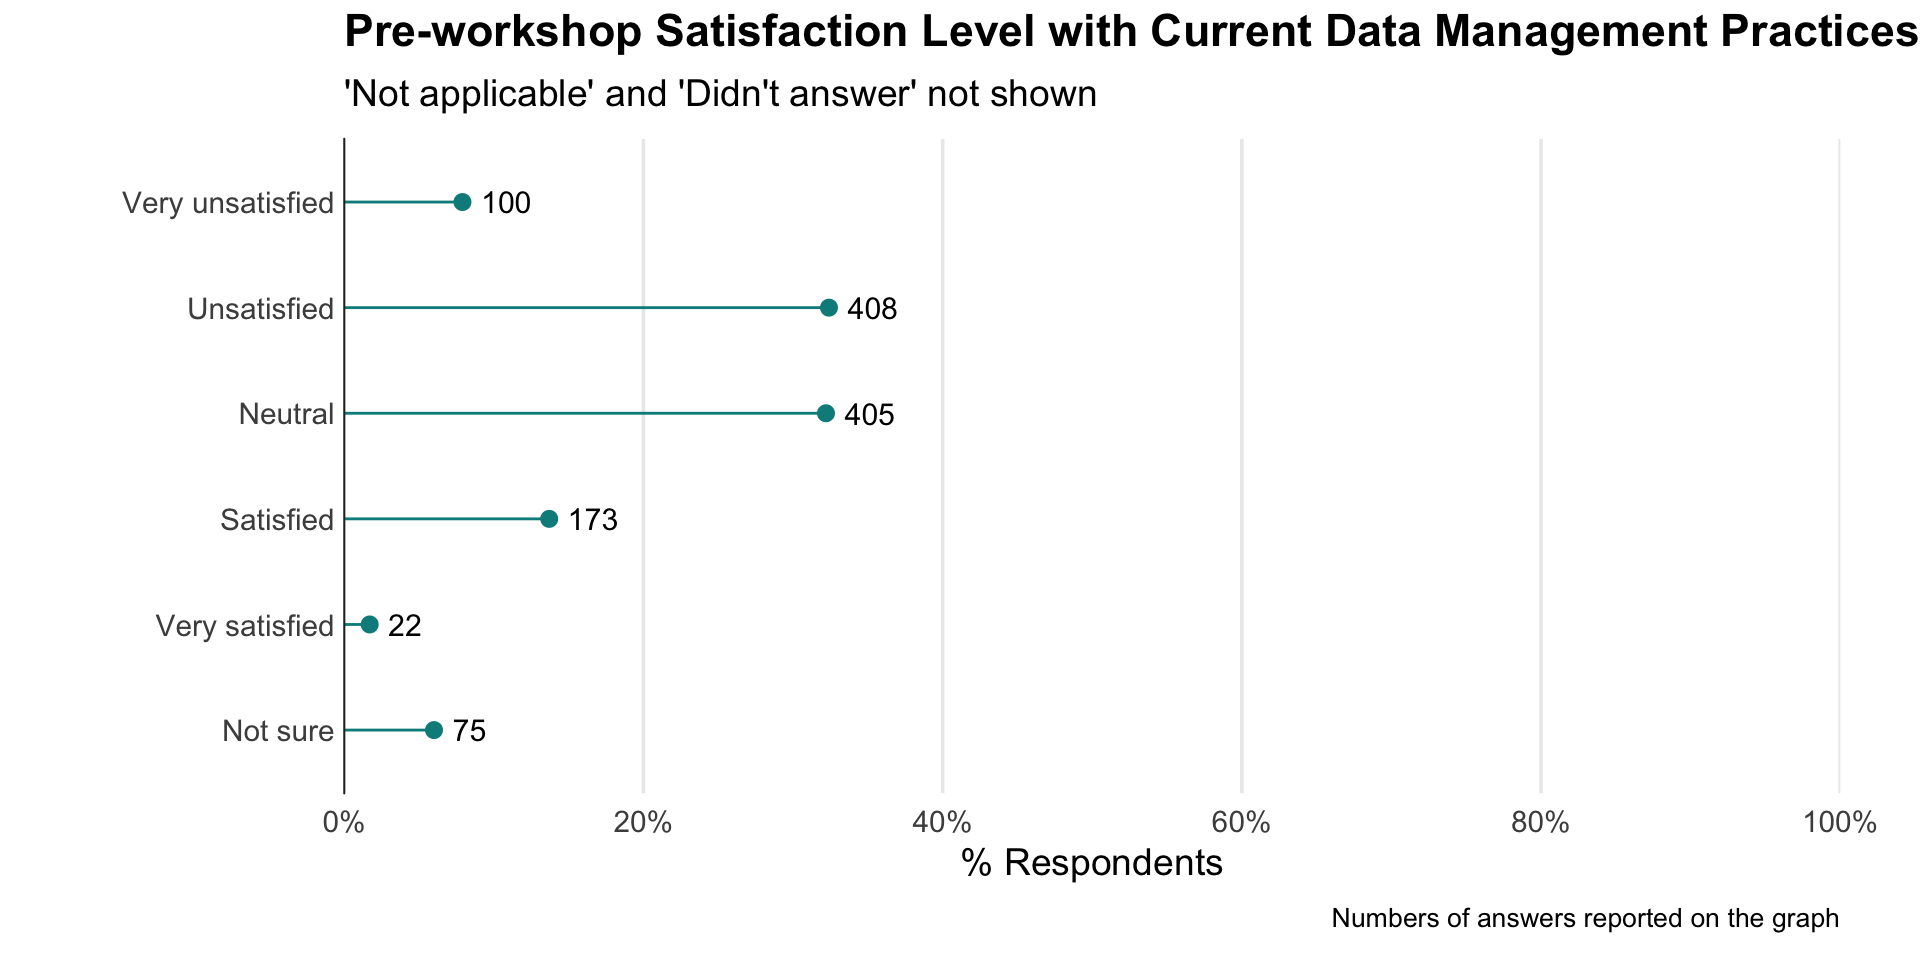
\includegraphics[width=\maxwidth]{../figures/dc-satisfaction-level-plot-1}

The majority (72.5\%) of Data Carpentry's respondents are either
unsatisfied or feel neutral with their current data management
practices. By data management practices, we include behaviors such as
keeping your raw data raw, reusing code, and using databases, queries,
and scripts to manage large data sets.

\subsubsection{How often do our workshop participants program before
attending our
workshops?}\label{how-often-do-our-workshop-participants-program-before-attending-our-workshops}

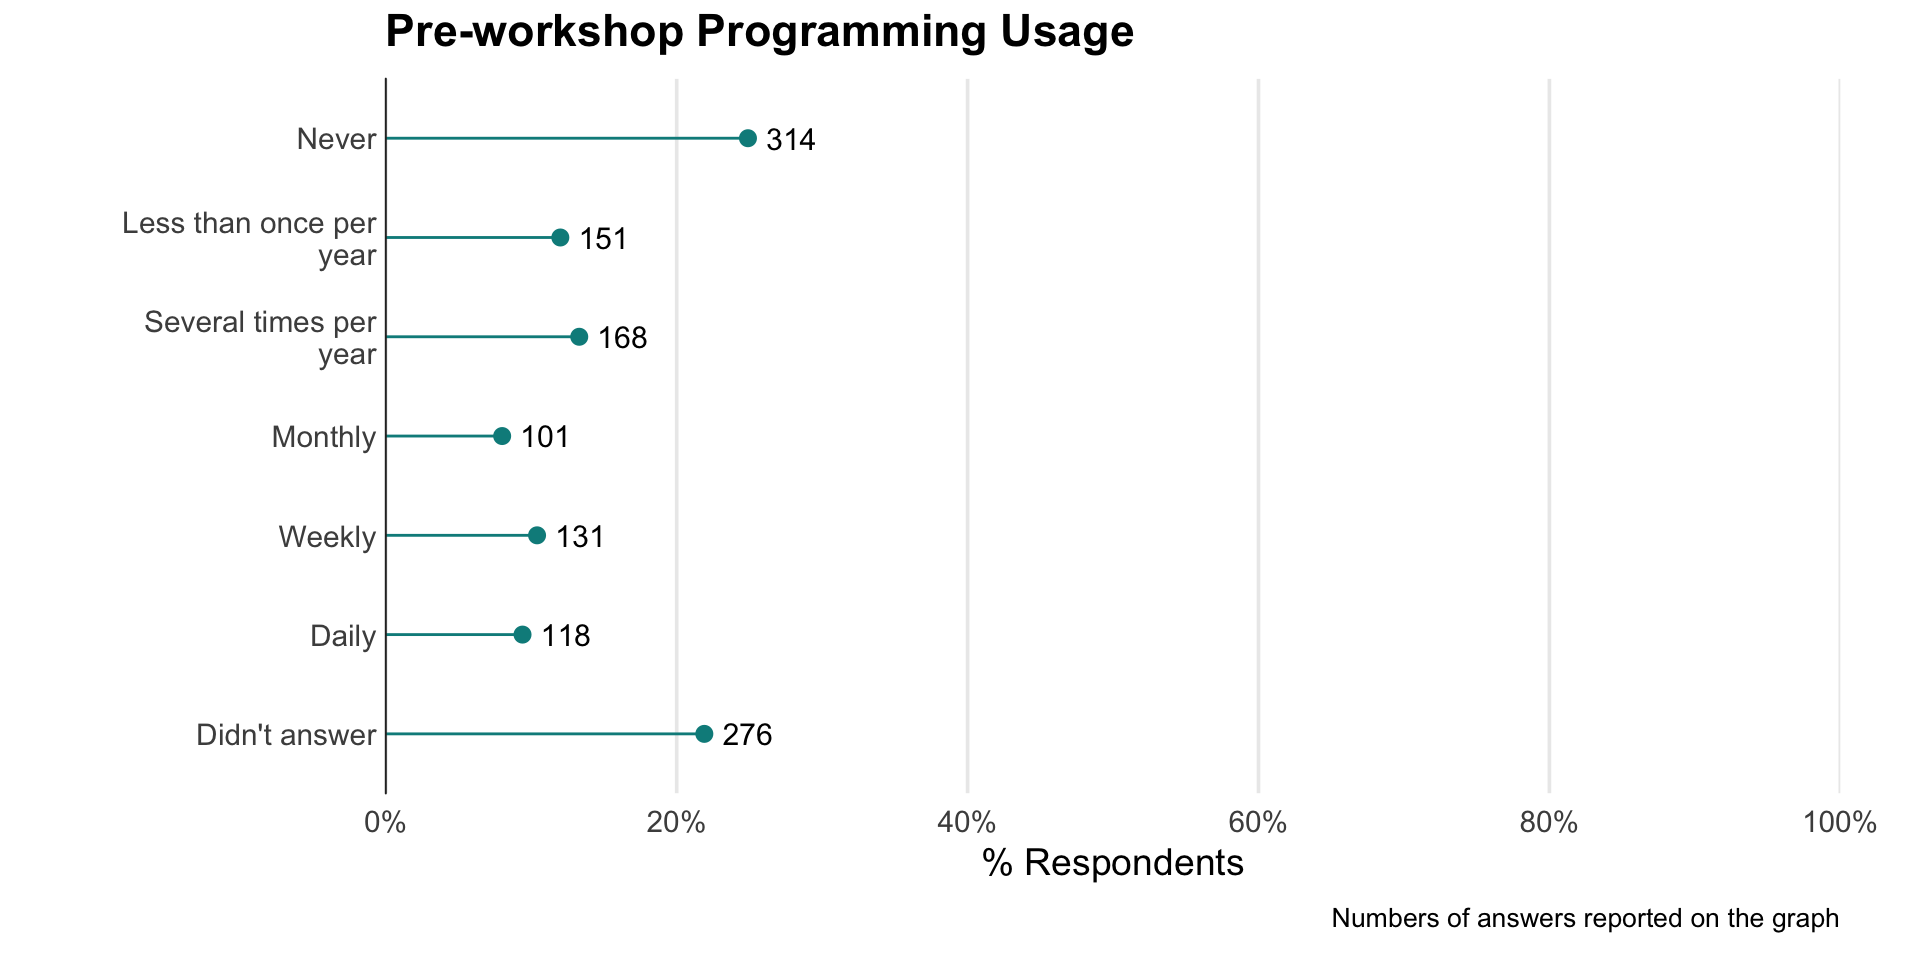
\includegraphics[width=\maxwidth]{../figures/dc-programming-level-plot-1}

In terms of current programming usage, 36.9\% of learners either never
use programming, use programming less than once per year, or no more
than several times per year. Only 9.4\% program on a daily basis. This
is no surprise, as Data Carpentry workshops are intended for novices.

\begin{longtable}[]{@{}lrr@{}}
\toprule
How respondents find out about Data Carpentry workshops (n =1243) & n &
\%\tabularnewline
\midrule
\endhead
Received an email about the workshop & 802 & 64.5\tabularnewline
My friend/colleague told me about it & 324 & 26.1\tabularnewline
My advisor/supervisor told me about it & 244 & 19.6\tabularnewline
Read about it in a newsletter or university web site & 85 &
6.8\tabularnewline
Other & 49 & 3.9\tabularnewline
Other web site & 20 & 1.6\tabularnewline
Twitter or other social media & 17 & 1.4\tabularnewline
\bottomrule
\end{longtable}

\begin{longtable}[]{@{}lrr@{}}
\toprule
\begin{minipage}[b]{0.78\columnwidth}\raggedright\strut
How respondents find out about Software Carpentry workshops (n =
10677)\strut
\end{minipage} & \begin{minipage}[b]{0.06\columnwidth}\raggedleft\strut
n\strut
\end{minipage} & \begin{minipage}[b]{0.06\columnwidth}\raggedleft\strut
\%\strut
\end{minipage}\tabularnewline
\midrule
\endhead
\begin{minipage}[t]{0.78\columnwidth}\raggedright\strut
Institution mailing list or flyer\strut
\end{minipage} & \begin{minipage}[t]{0.06\columnwidth}\raggedleft\strut
5143\strut
\end{minipage} & \begin{minipage}[t]{0.06\columnwidth}\raggedleft\strut
48.2\strut
\end{minipage}\tabularnewline
\begin{minipage}[t]{0.78\columnwidth}\raggedright\strut
Friend/colleague\strut
\end{minipage} & \begin{minipage}[t]{0.06\columnwidth}\raggedleft\strut
4810\strut
\end{minipage} & \begin{minipage}[t]{0.06\columnwidth}\raggedleft\strut
45.1\strut
\end{minipage}\tabularnewline
\begin{minipage}[t]{0.78\columnwidth}\raggedright\strut
Other\strut
\end{minipage} & \begin{minipage}[t]{0.06\columnwidth}\raggedleft\strut
758\strut
\end{minipage} & \begin{minipage}[t]{0.06\columnwidth}\raggedleft\strut
7.1\strut
\end{minipage}\tabularnewline
\begin{minipage}[t]{0.78\columnwidth}\raggedright\strut
Conference/meeting/seminar\strut
\end{minipage} & \begin{minipage}[t]{0.06\columnwidth}\raggedleft\strut
637\strut
\end{minipage} & \begin{minipage}[t]{0.06\columnwidth}\raggedleft\strut
6.0\strut
\end{minipage}\tabularnewline
\begin{minipage}[t]{0.78\columnwidth}\raggedright\strut
Our website\strut
\end{minipage} & \begin{minipage}[t]{0.06\columnwidth}\raggedleft\strut
356\strut
\end{minipage} & \begin{minipage}[t]{0.06\columnwidth}\raggedleft\strut
3.3\strut
\end{minipage}\tabularnewline
\begin{minipage}[t]{0.78\columnwidth}\raggedright\strut
Funding organization or program officer\strut
\end{minipage} & \begin{minipage}[t]{0.06\columnwidth}\raggedleft\strut
355\strut
\end{minipage} & \begin{minipage}[t]{0.06\columnwidth}\raggedleft\strut
3.3\strut
\end{minipage}\tabularnewline
\begin{minipage}[t]{0.78\columnwidth}\raggedright\strut
Social Media (Twitter, Facebook, etc.)\strut
\end{minipage} & \begin{minipage}[t]{0.06\columnwidth}\raggedleft\strut
293\strut
\end{minipage} & \begin{minipage}[t]{0.06\columnwidth}\raggedleft\strut
2.7\strut
\end{minipage}\tabularnewline
\begin{minipage}[t]{0.78\columnwidth}\raggedright\strut
Journal or publication\strut
\end{minipage} & \begin{minipage}[t]{0.06\columnwidth}\raggedleft\strut
37\strut
\end{minipage} & \begin{minipage}[t]{0.06\columnwidth}\raggedleft\strut
0.3\strut
\end{minipage}\tabularnewline
\bottomrule
\end{longtable}

Data Carpentry and Software Carpentry workshop participants often find
out about our workshops through institutional mailing lists (64.5\% and
48.2\% respectively). However, ``word-of-mouth'' recommendations also
play a significant role in populating workshops.

In summary, both Data and Software Carpentry workshop respondents attend
workshops to learn about or improve upon their current data management
and analysis skills.

\subsection{Workshop Type}\label{workshop-type}

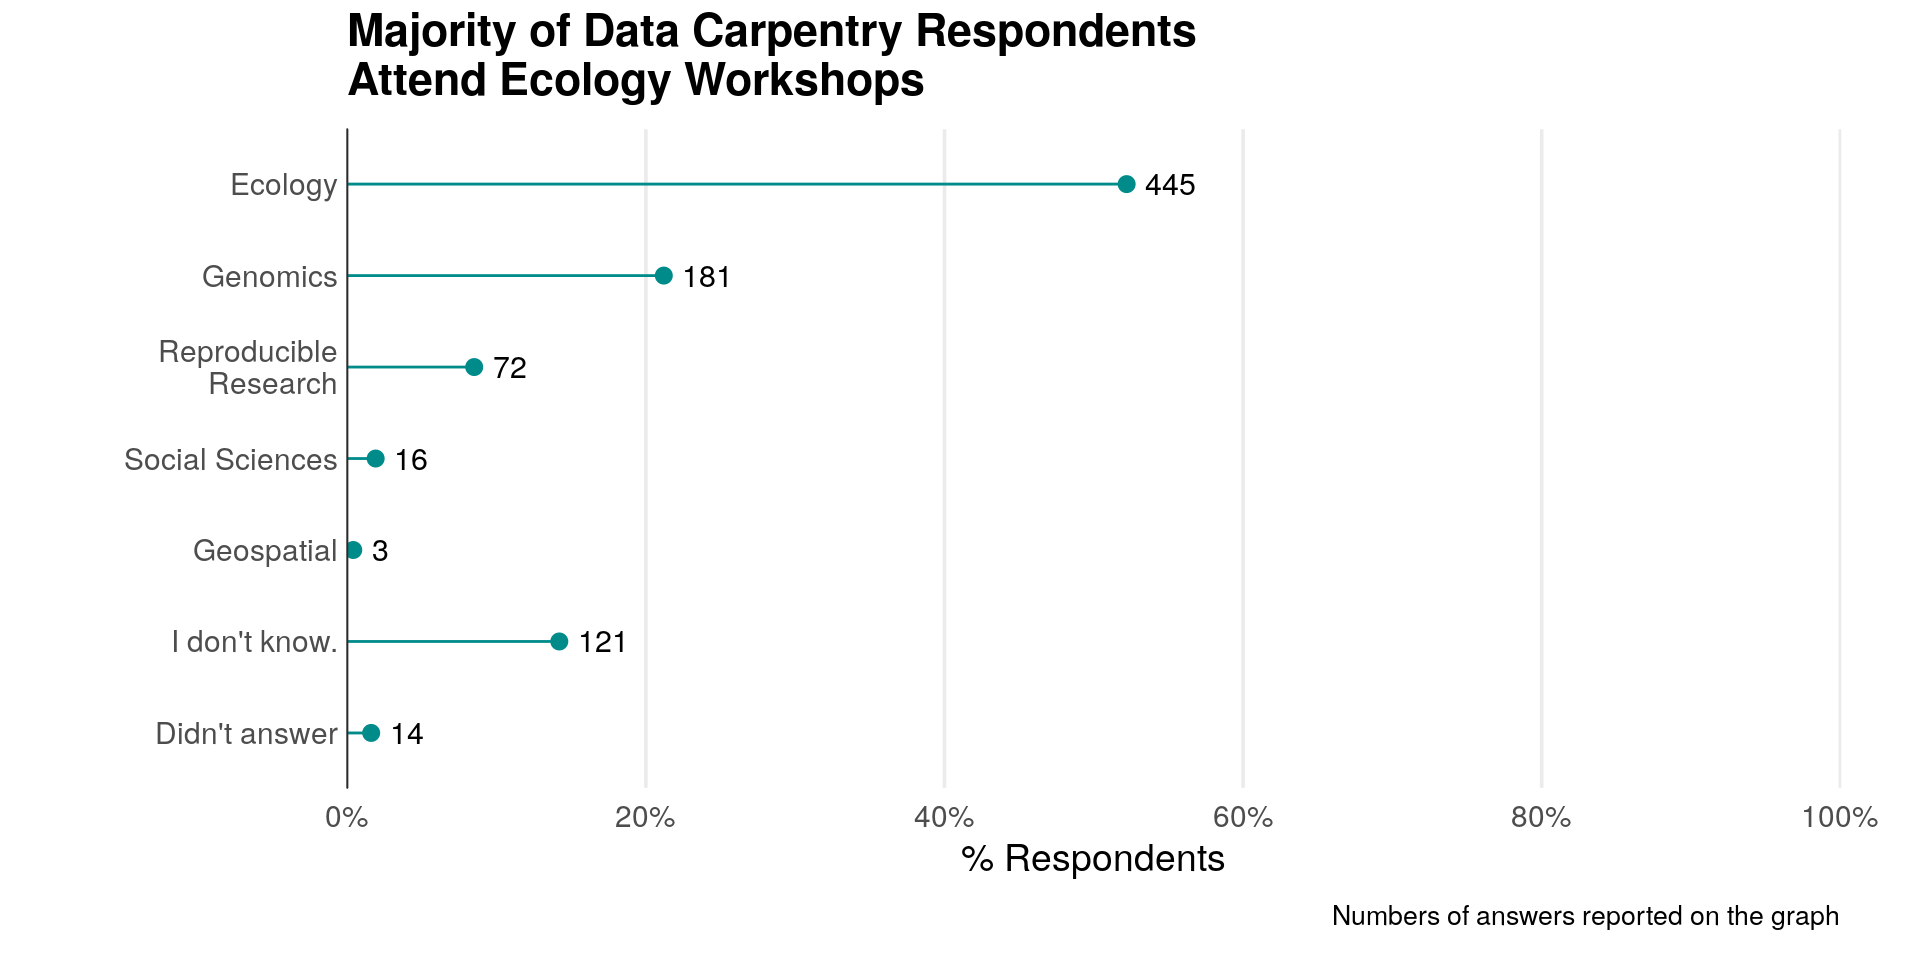
\includegraphics[width=\maxwidth]{../figures/dc-workshop-type-plot-1}

\begin{longtable}[]{@{}lrr@{}}
\toprule
Data Carpentry: Language Covered in Workshops & n & \%\tabularnewline
\midrule
\endhead
R & 614 & 72.1\tabularnewline
Python & 118 & 13.8\tabularnewline
Didn't answer & 58 & 6.8\tabularnewline
Neither & 57 & 6.7\tabularnewline
I don't know./I don't remember. & 5 & 0.6\tabularnewline
\bottomrule
\end{longtable}

As previously mentioned, Data Carpentry workshops are domain-specific,
and curricula include Ecology, Genomics, Geospatial, Social Sciences,
and Reproducible Research. 72.1\% of respondents learned R in their
workshop, while 13.8\% learned Python.

\subsection{Perception of Workshop Environment and
Experience}\label{perception-of-workshop-environment-and-experience}

\subsubsection{Comfort of the
environment}\label{comfort-of-the-environment}

The Carpentries is committed to making participation in our workshops a
harassment-free experience for everyone, regardless of who learners are,
where they are from, or what their experience is with the tools we
teach. We establish norms for interaction by having, discussing, and
enforcing a Code of Conduct so that our workshops provide open and
inclusive learning environments. 79\% of Data Carpentry respondents
either agree or strongly agree that they felt comfortable learning in
their workshop environment, and 87.1\% of Software Carpentry's
respondents agreed or strongly agreed that the workshop atmosphere was
welcoming.

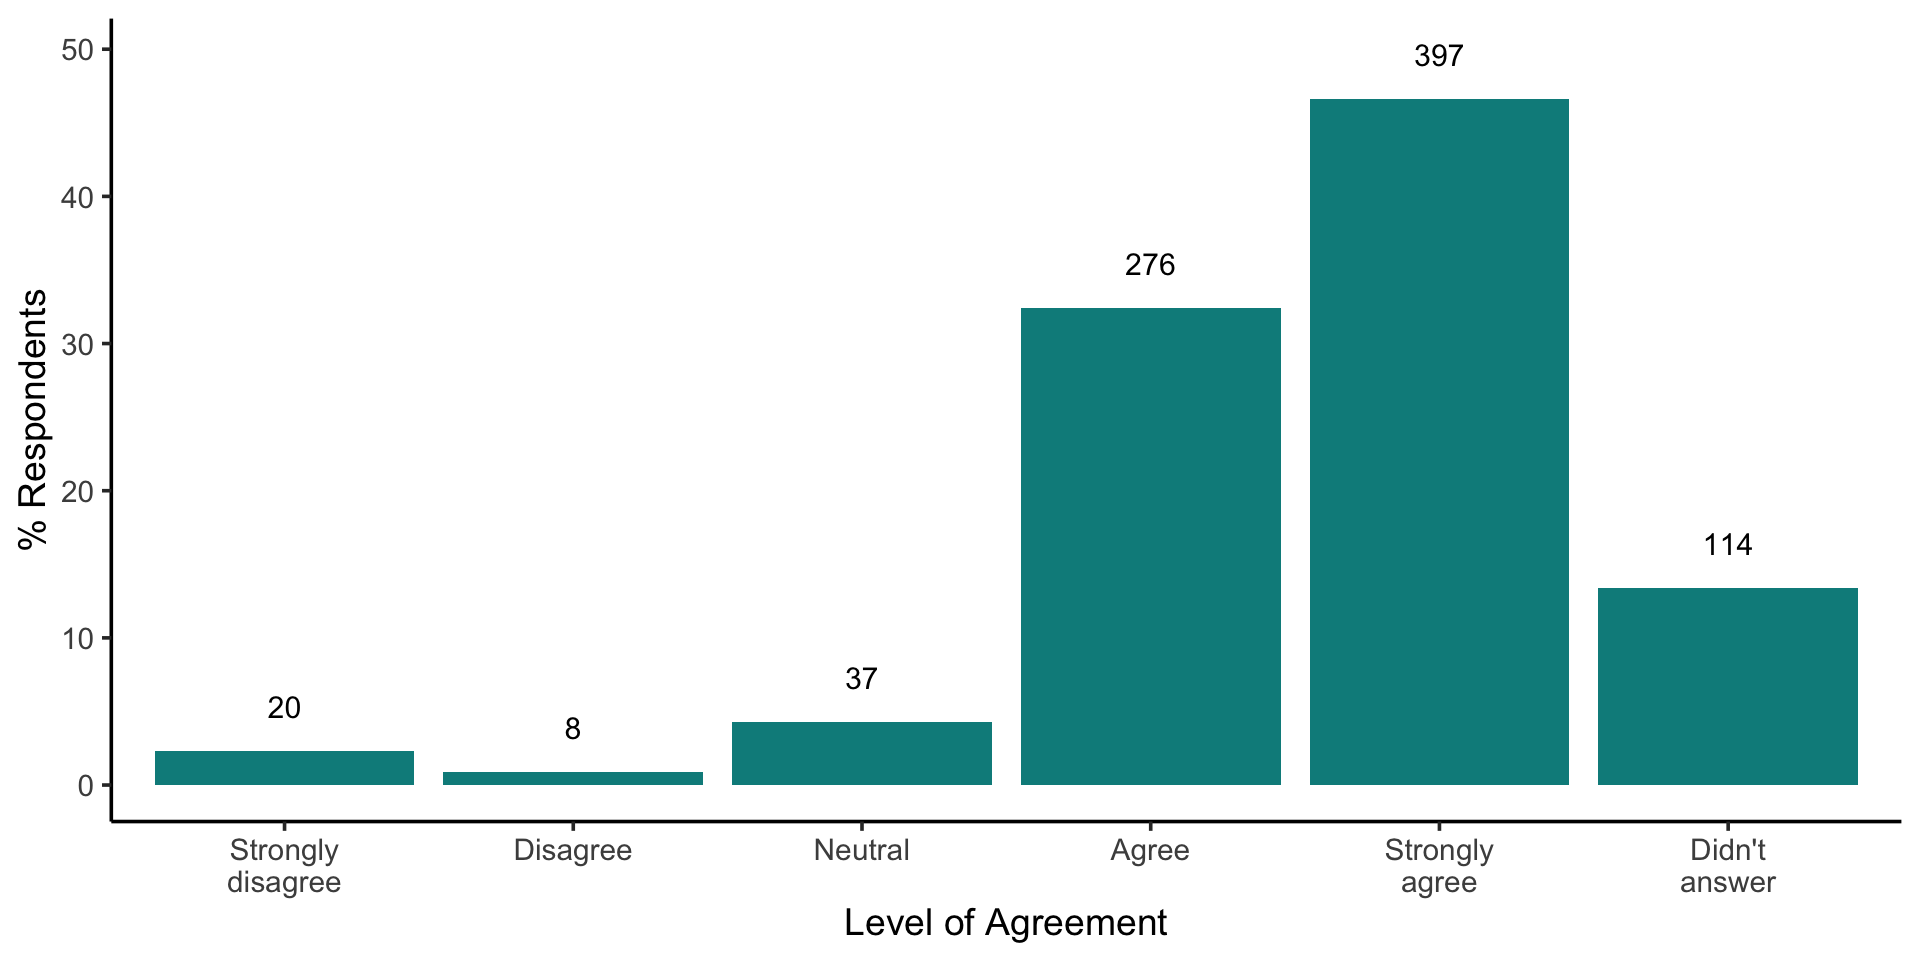
\includegraphics[width=\maxwidth]{../figures/dc-post-workshop-comfortable-environment-1}

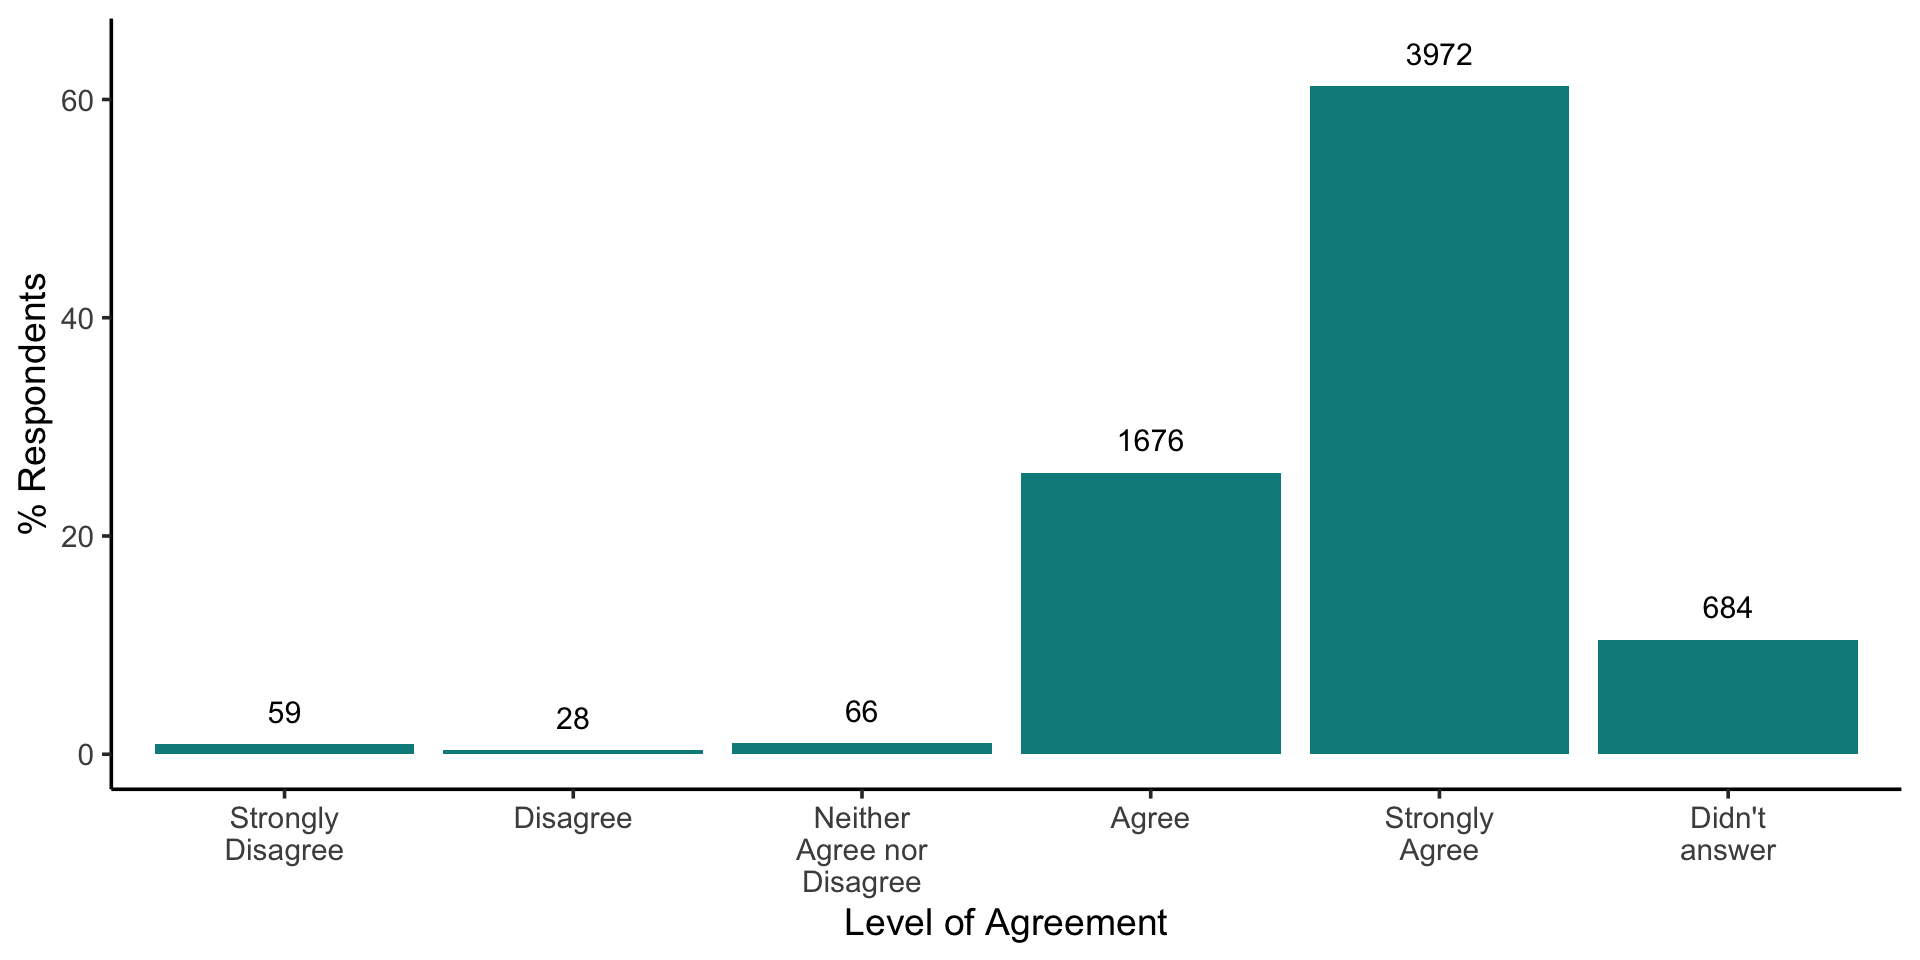
\includegraphics[width=\maxwidth]{../figures/swc-post-workshop-environment-1}

\subsubsection{Interaction with Instructors and
Helpers}\label{interaction-with-instructors-and-helpers}

Data Carpentry respondents were asked to rate their level of agreement
with several statements regarding their instructors' knowledge,
instructional method, and enthusiasm. Their responses are in the figure
below, and axis labels correspond to the statements as follows:

\begin{itemize}
\tightlist
\item
  \textbf{Instructors Knowledge}: The instructors were knowledgeable
  about the material being taught.
\item
  \textbf{Instructors Interacting}: I felt comfortable interacting with
  the instructors.
\item
  \textbf{Instructors Enthusiastic}: The instructors were enthusiastic
  about the workshop.
\item
  \textbf{Instructors Clear Answers}: I was able to get clear answers to
  my questions from the instructors.
\end{itemize}

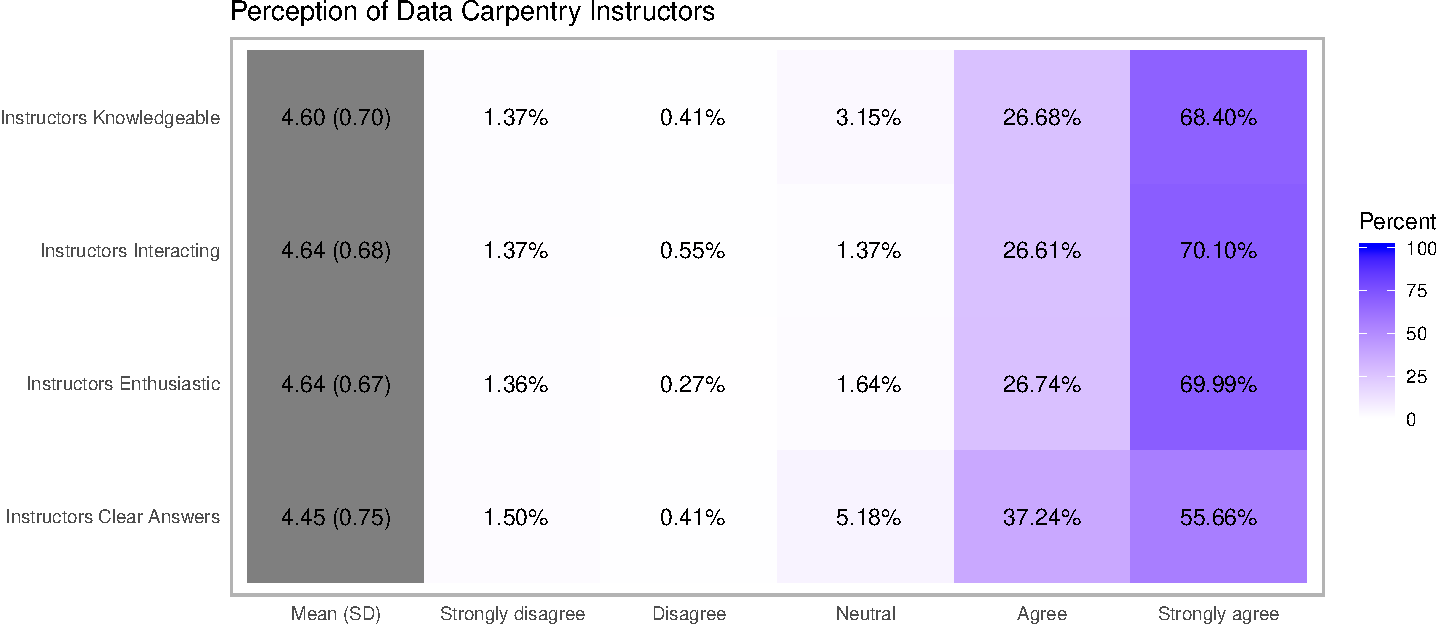
\includegraphics[width=\maxwidth]{../figures/dc-perception-instructors-heatmap-1}

The largest impact we see is that 96.2\% of respondents said they felt
comfortable interacting with the instructors. We know that our
instructors \emph{are} the reason why our workshops are so
well-received. It is also great to see that 94.8\% and 96.7\% of
respondents felt our instructors were knowledgeable about the material
being taught, and were enthusiastic about the workshop, respectively.
Lastly, 92.9\% of respondents felt they were able to get clear answers
to their questions from their instructors.

Software Carpentry respondents were asked to rate how they felt
instructors and helpers worked as a team, based on the following
criteria:

\begin{itemize}
\tightlist
\item
  \textbf{Considerate}: Instructors/Helpers were considerate.
\item
  \textbf{Enthusiastic}: Instructors/Helpers were enthusiastic.
\item
  \textbf{Clear Answers}: Instructors/Helpers gave clear answers to your
  questions.
\item
  \textbf{Communicators}: Instructors/Helpers were good communicators.
\end{itemize}

The two neutral centered plots below provide an analysis of respondent's
answers for both instructors and helpers.

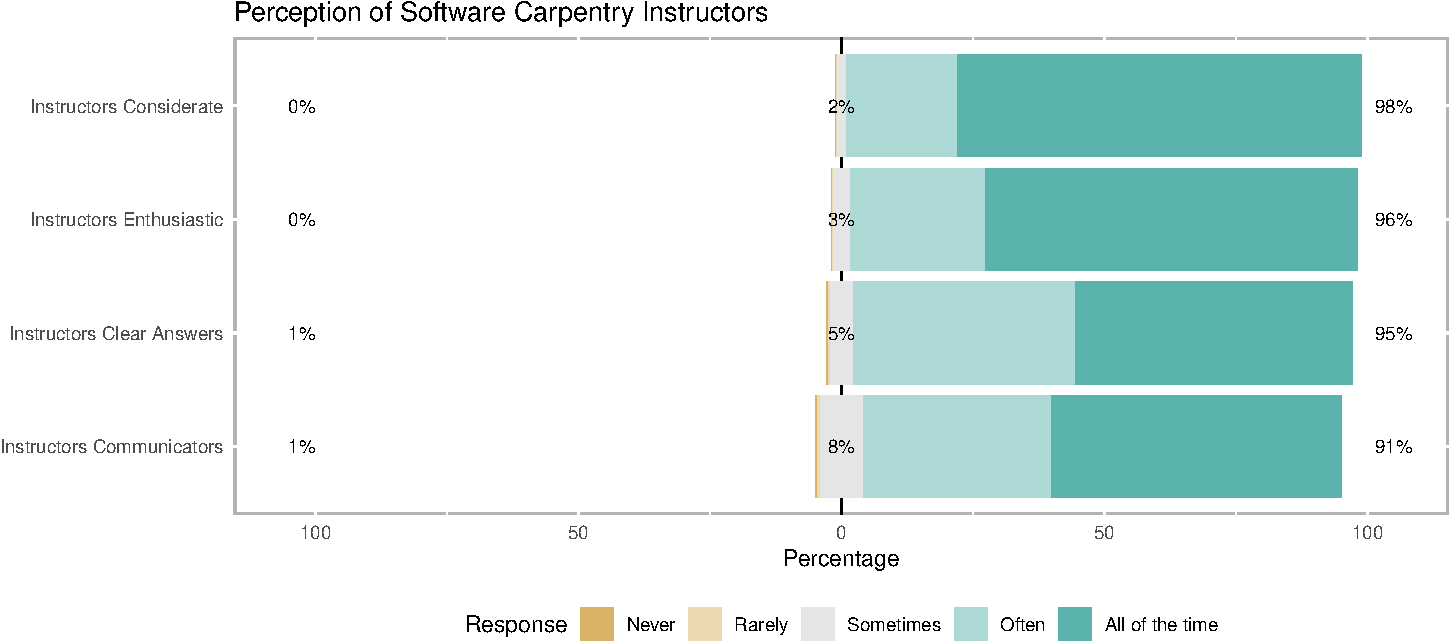
\includegraphics[width=\maxwidth]{../figures/swc-perception-instructors-1}

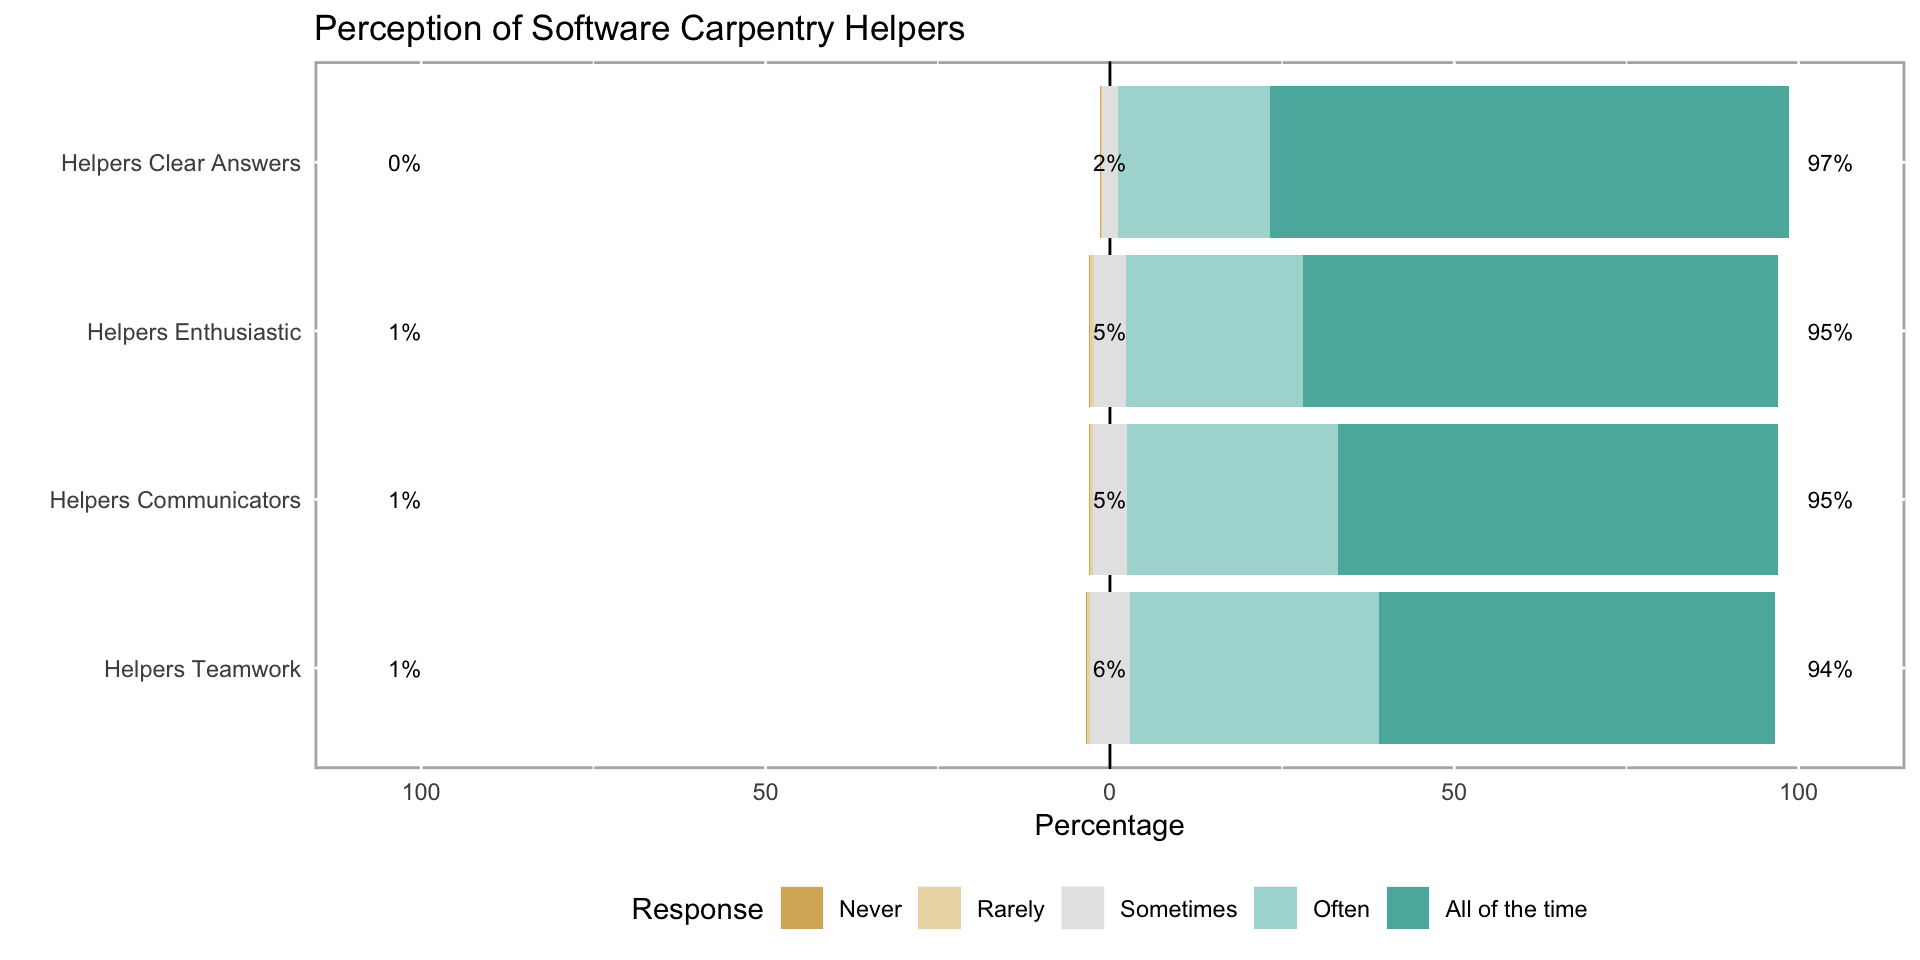
\includegraphics[width=\maxwidth]{../figures/swc-perception-helpers-1}

From the figures above, we see that Software Carpentry instructors and
helpers are considerate, enthusiastic, give clear answers to questions,
and are good communicators. As a whole, our instructors work as a team
and are successful in creating a warm and welcoming workshop
environment.

\subsection{Applicability of the skills
learned}\label{applicability-of-the-skills-learned}

One of the goals for Data Carpentry's lessons is that learners are able
to immediately apply what they learned at the workshop. The figure below
shows that 65.2\% either agree or strongly agree that they were able to
apply what they learned immediately.

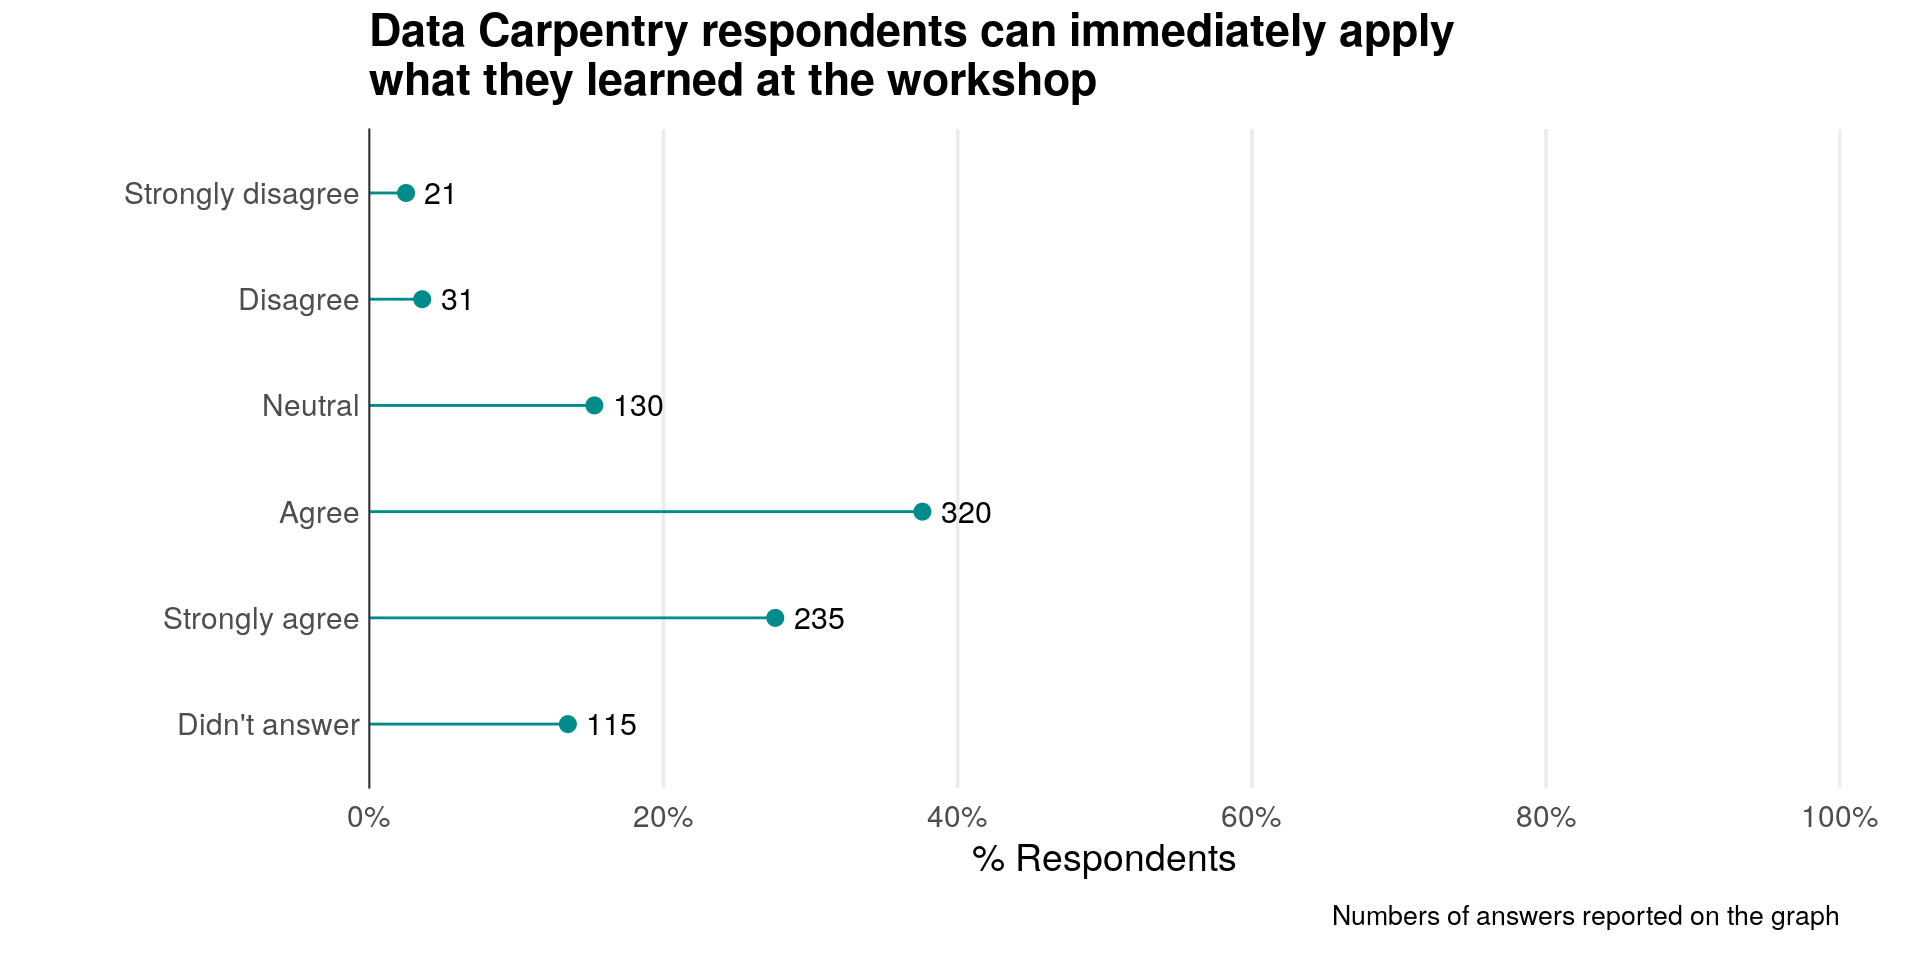
\includegraphics[width=\maxwidth]{../figures/dc-skill-applicability-plot-1}

\subsection{Was the information covered in the workshops
new?}\label{was-the-information-covered-in-the-workshops-new}

As the majority of Software Carpentry learners attend workshops to learn
new skills, it is great to see that 47.2\% of learners either learned
mostly or all new information during the workshop, while another 16.9\%
learned something new.

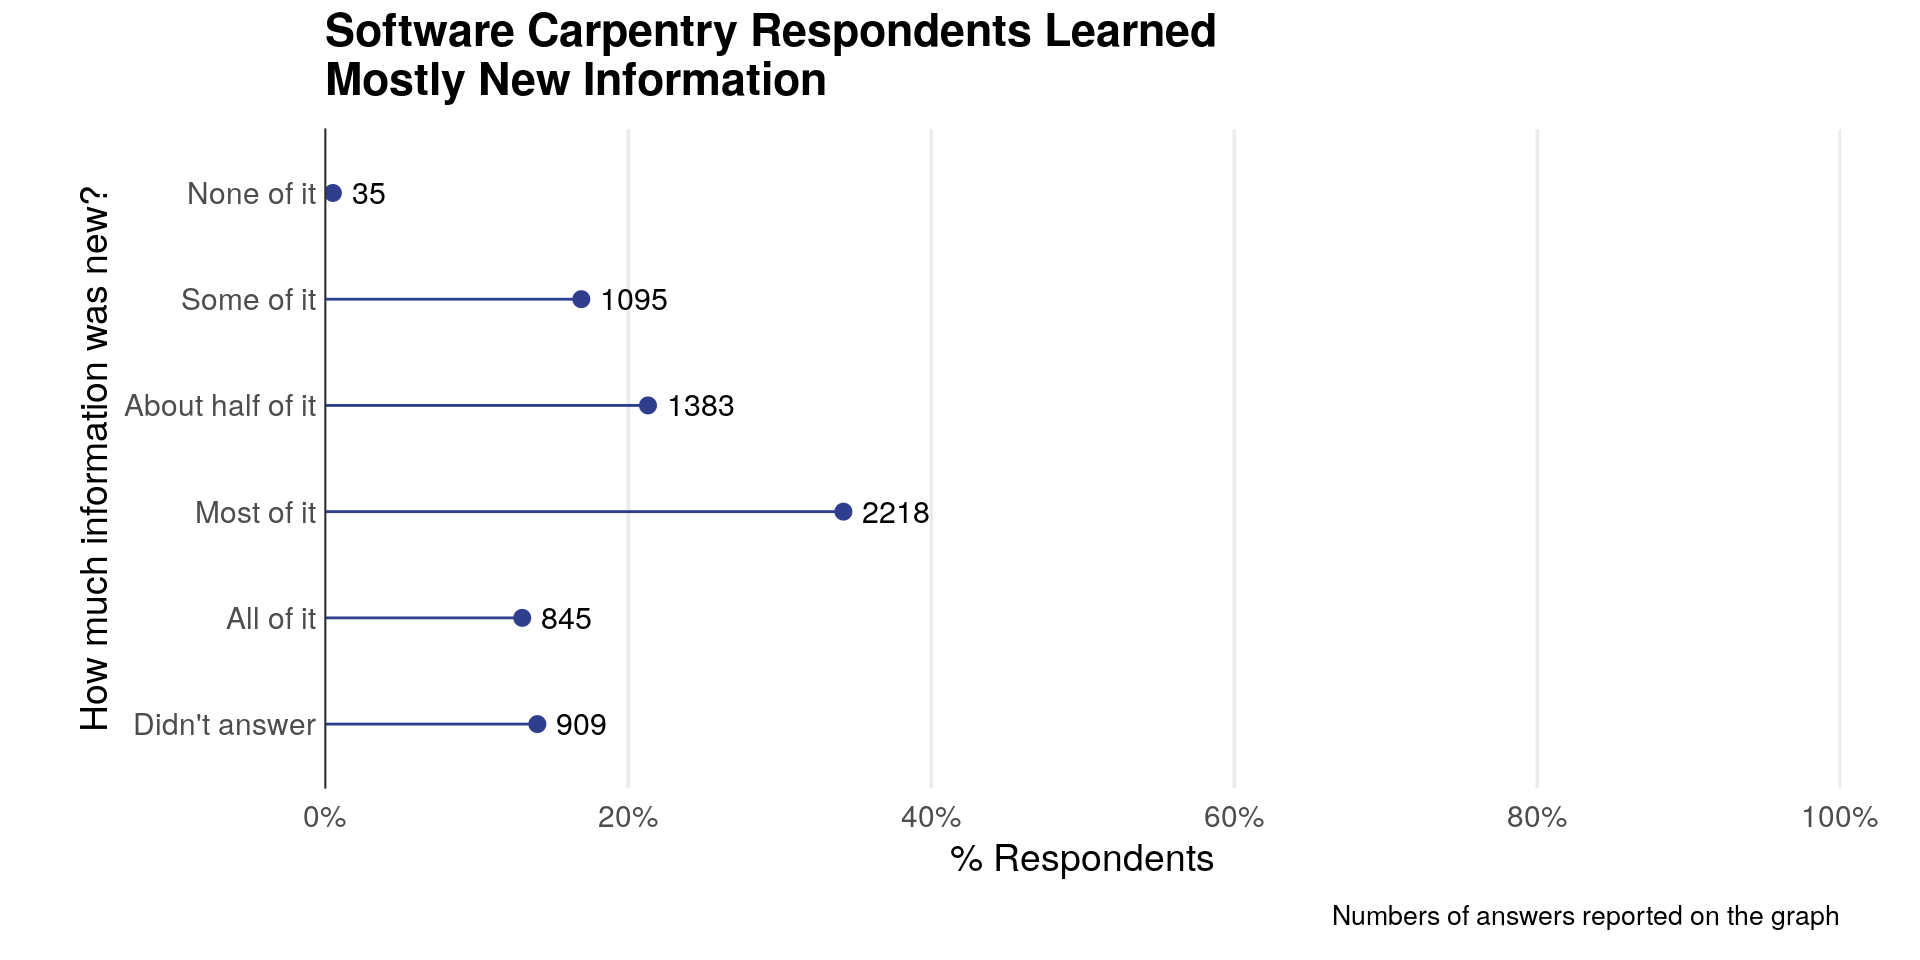
\includegraphics[width=\maxwidth]{../figures/swc-new-information-plot-1}

\subsection{Workshop Experience}\label{workshop-experience}

\begin{longtable}[]{@{}lrr@{}}
\toprule
Data Carpentry Respondents Having Accessibility Issues & n &
\%\tabularnewline
\midrule
\endhead
Yes & 79 & 9.3\tabularnewline
No & 654 & 76.8\tabularnewline
Didn't answer & 119 & 14.0\tabularnewline
\bottomrule
\end{longtable}

We want to be proactive in ensuring learners have access to whatever
they need to participate in a workshop. Both Data Carpentry and Software
Carpentry learners were asked to inform workshop organizers if there was
anything they needed to make their workshop experience better. Data
Carpentry's respondents were asked if they had accessibility issues, and
9.3\% reported they did. After reading the open-ended responses, we can
see that the issues were related to not being able to hear and/or see in
the back of the room. The Instructor Training Team has been made aware
of this, and will be making recommendations.

\subsection{Net Promoter Score}\label{net-promoter-score}

We use the \href{https://en.wikipedia.org/wiki/Net_Promoter}{Net
Promoter Score} to measure learners' likelihood of recommending
workshops to a friend or colleague. The scoring for this question is on
a 0 to 100 scale. Respondents scoring from 0 to 64 are labeled
\emph{Detractors}, and are believed to be less likely to recommend a
workshop. Those who respond with a score of 85 to 100 are called
\emph{Promoters}, and are considered likely to recommend a workshop.
Respondents between 65 and 84 are labeled \emph{Passives}, and their
behavior falls between Promoters and Detractors.

\begin{longtable}[]{@{}lrr@{}}
\toprule
Data Carpentry Net Promoter Score & n & \%\tabularnewline
\midrule
\endhead
Detractor & 32 & 3.8\tabularnewline
Passive & 131 & 15.4\tabularnewline
Promoter & 565 & 66.3\tabularnewline
Didn't answer & 124 & 14.6\tabularnewline
\bottomrule
\end{longtable}

77.6\% of Data Carpentry respondents who answered this question are
promoters (i.e.~would recommend a workshop).

For Software Carpentry respondents who answered this questions, 56.9\%
are promoters.

In summary, Data Carpentry and Software Carpentry workshops provide a
warm and welcoming environment, whether learners are brand new to
programming or have some experience. Attendees are recommending
workshops to their friends and colleagues, and we know that our
instructors and helpers are the major reason why.

\subsection{Effect of Workshops on Learners Self-Reported Perspectives:
Skills \&
Confidence}\label{effect-of-workshops-on-learners-self-reported-perspectives-skills-confidence}

Learners were asked to rate their level of agreement with the following
statements related to Data Carpentry's workshop goals and learning
objectives. The figure below provides a visual representation of their
responses, comparing them before the workshop and after the workshop.
Axis labels and the corresponding question are organized around 3 themes
as follows:

\begin{itemize}
\tightlist
\item
  Efficiency:

  \begin{itemize}
  \tightlist
  \item
    \textbf{Write Program}: I can write a small program/script/macro to
    solve a problem in my own work.
  \item
    \textbf{Programming Efficient}: Using a programming language (like R
    or Python) can make me more efficient at working with data.
  \end{itemize}
\item
  Reproducibility:

  \begin{itemize}
  \tightlist
  \item
    \textbf{Raw Data}: Having access to the original, raw data is
    important to be able to repeat an analysis.
  \item
    \textbf{Analyses Easier}: Using a programming language (like R or
    Python) can make my analyses easier to reproduce.
  \end{itemize}
\item
  Self-efficacy

  \begin{itemize}
  \tightlist
  \item
    \textbf{Search Online}: I know how to search for answers to my
    technical questions online.
  \item
    \textbf{Overcome Problem}: While working on a programming project,
    if I get stuck, I can find ways of overcoming the problem.
  \item
    \textbf{Programming Confident}: I am confident in my ability to make
    use of programming software to work with data.
  \end{itemize}
\end{itemize}

The scoring for the above factors ranges from strongly disagree (1) to
strongly agree (5).

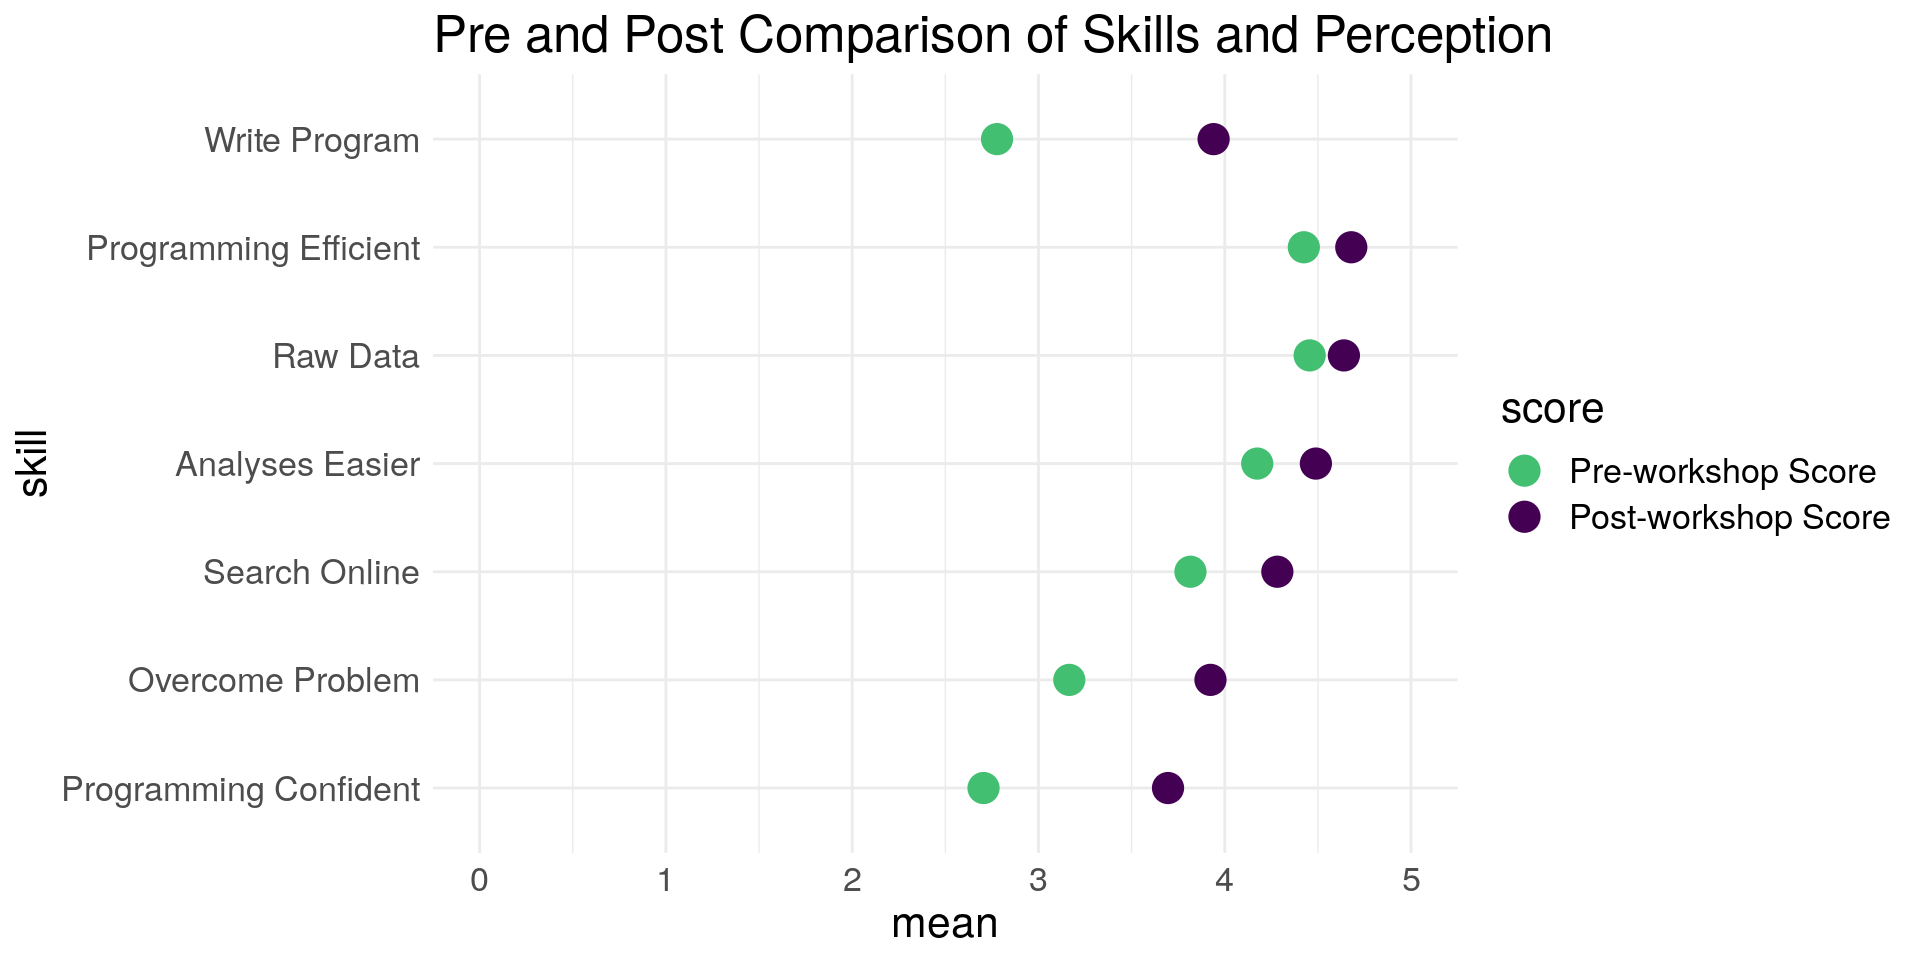
\includegraphics[width=\maxwidth]{../figures/dc-paired-data-mean-1}

The comparison above is paired, meaning, we are comparing those who
provided us with a unique identifier and who completed both the pre- and
post-workshop survey. This figure includes 411 responses. The data
shows, for multiple factors, a full point increase in mean score. We are
significantly impacting respondents' confidence in programming, ability
to write programs to solve problems, and ability to overcome problems if
they get stuck.

In the figures below, we show another representation of the pre- and
post-comparison of respondents skills and perspectives. The figures
below include the data for all learners, not only those who provided a
unique identifier \emph{and} took both the pre- and post-workshop
surveys. What we see is a shift in the distribution for each factor,
meaning, respondents' self-reported confidence and ability shifted in
positive directions.

The neutral centered graphs below provide an even clearer picture of the
shift in respondents' self-reported confidence and skills.

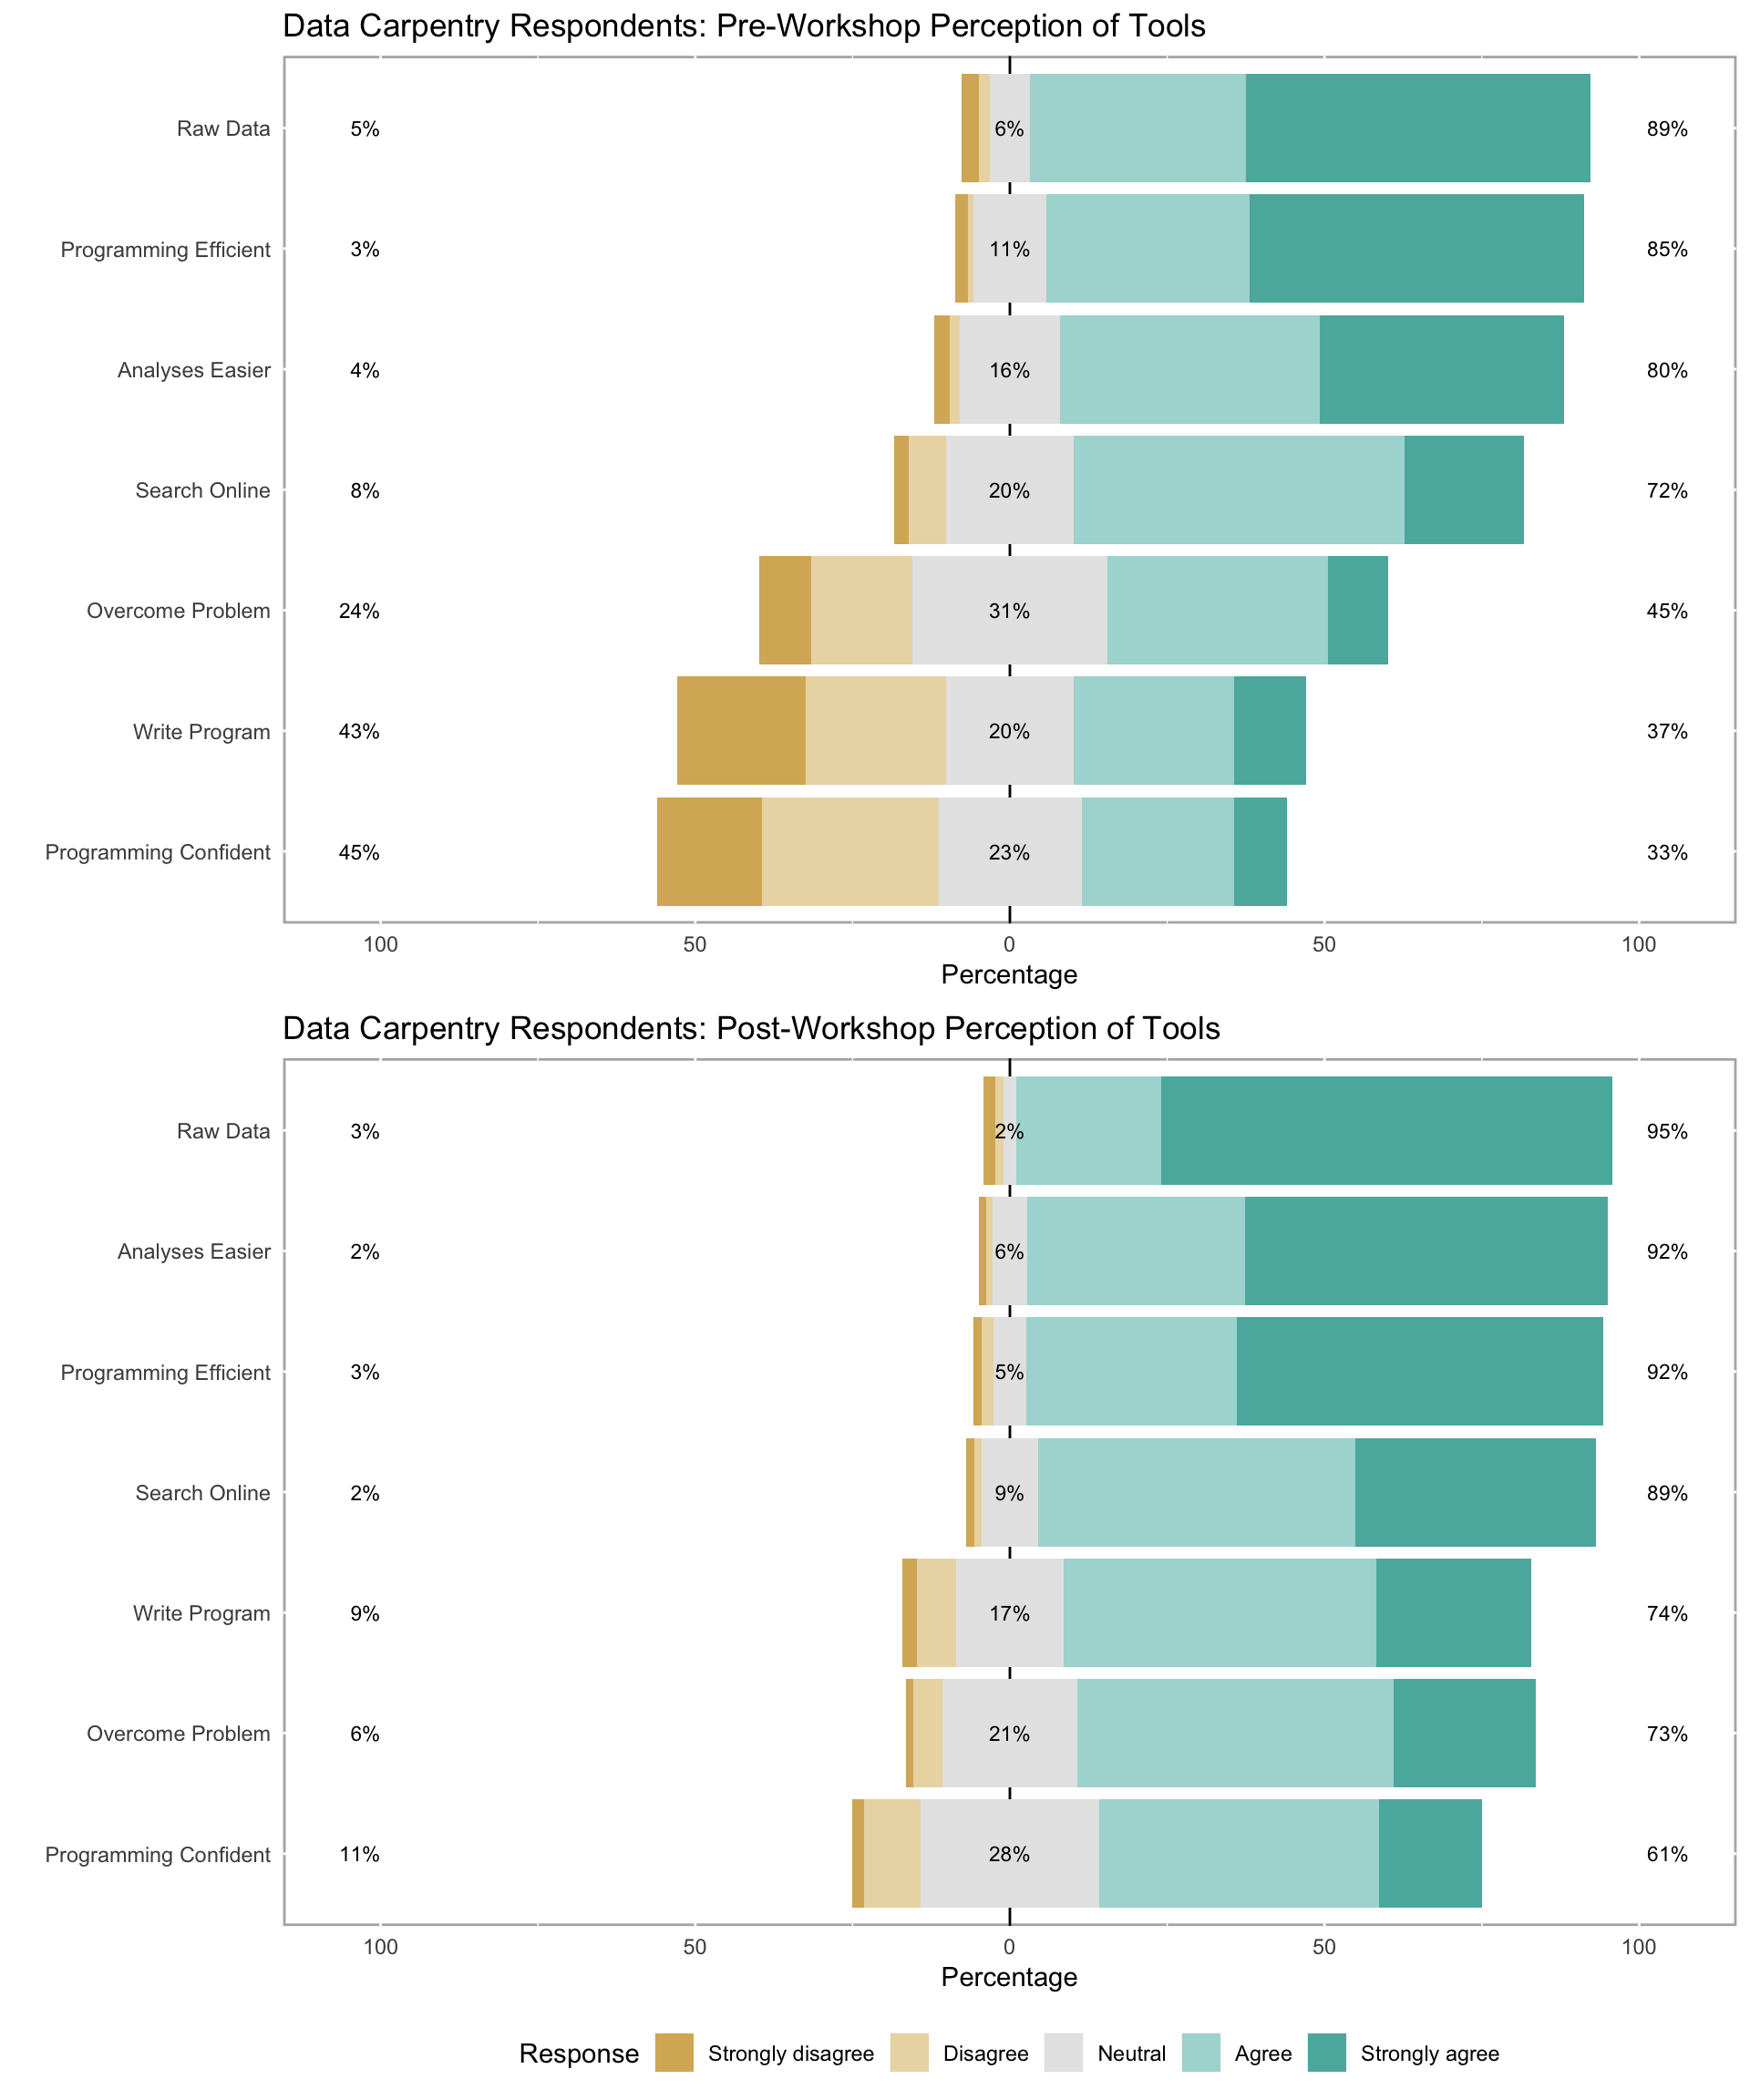
\includegraphics[width=\maxwidth]{../figures/dc-tools-perception-1}

It is interesting to see the shift in neutrality between the
pre-workshop scores and post-workshop scores, especially for
\emph{Programming Efficient}. There was a higher percentage of learners
beginning the workshop who felt programming with R or Python can make
them more efficient at working with data. Contrarily, confidence in
using programming to work with data increased from 33\% to 61\%.

Software Carpentry Respondents were asked to tell us about their
experience with these topics before the workshop:

\begin{itemize}
\tightlist
\item
  R
\item
  Unix Shell
\item
  SQL
\item
  Python
\item
  Version Control with Git
\end{itemize}

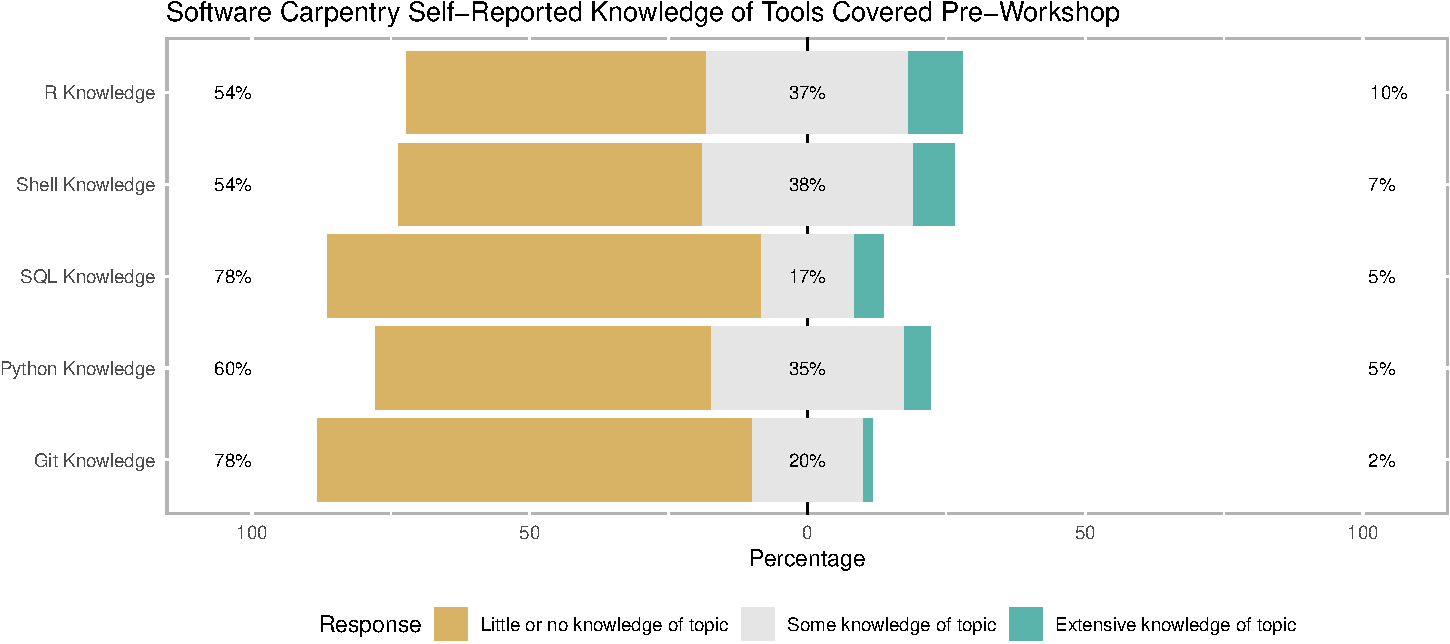
\includegraphics[width=\maxwidth]{../figures/swc-pre-tools-1}

From the figure, we see that learners consider themselves beginners from
the topics covered in our workshops. When asked their knowledge of the
tools covered in their workshops, learners rated their knowledge as
extensive from 2\% to 10\% for ``Git Knowledge'' and ``R Knowledge''.

The following is a comparison of Software Carpentry respondents'
knowledge about the tools before compared to after the workshop. We see
clearly that after the workshop, respondents' knowledge of Git, Python,
R, and the Unix Shell had increased a great deal.

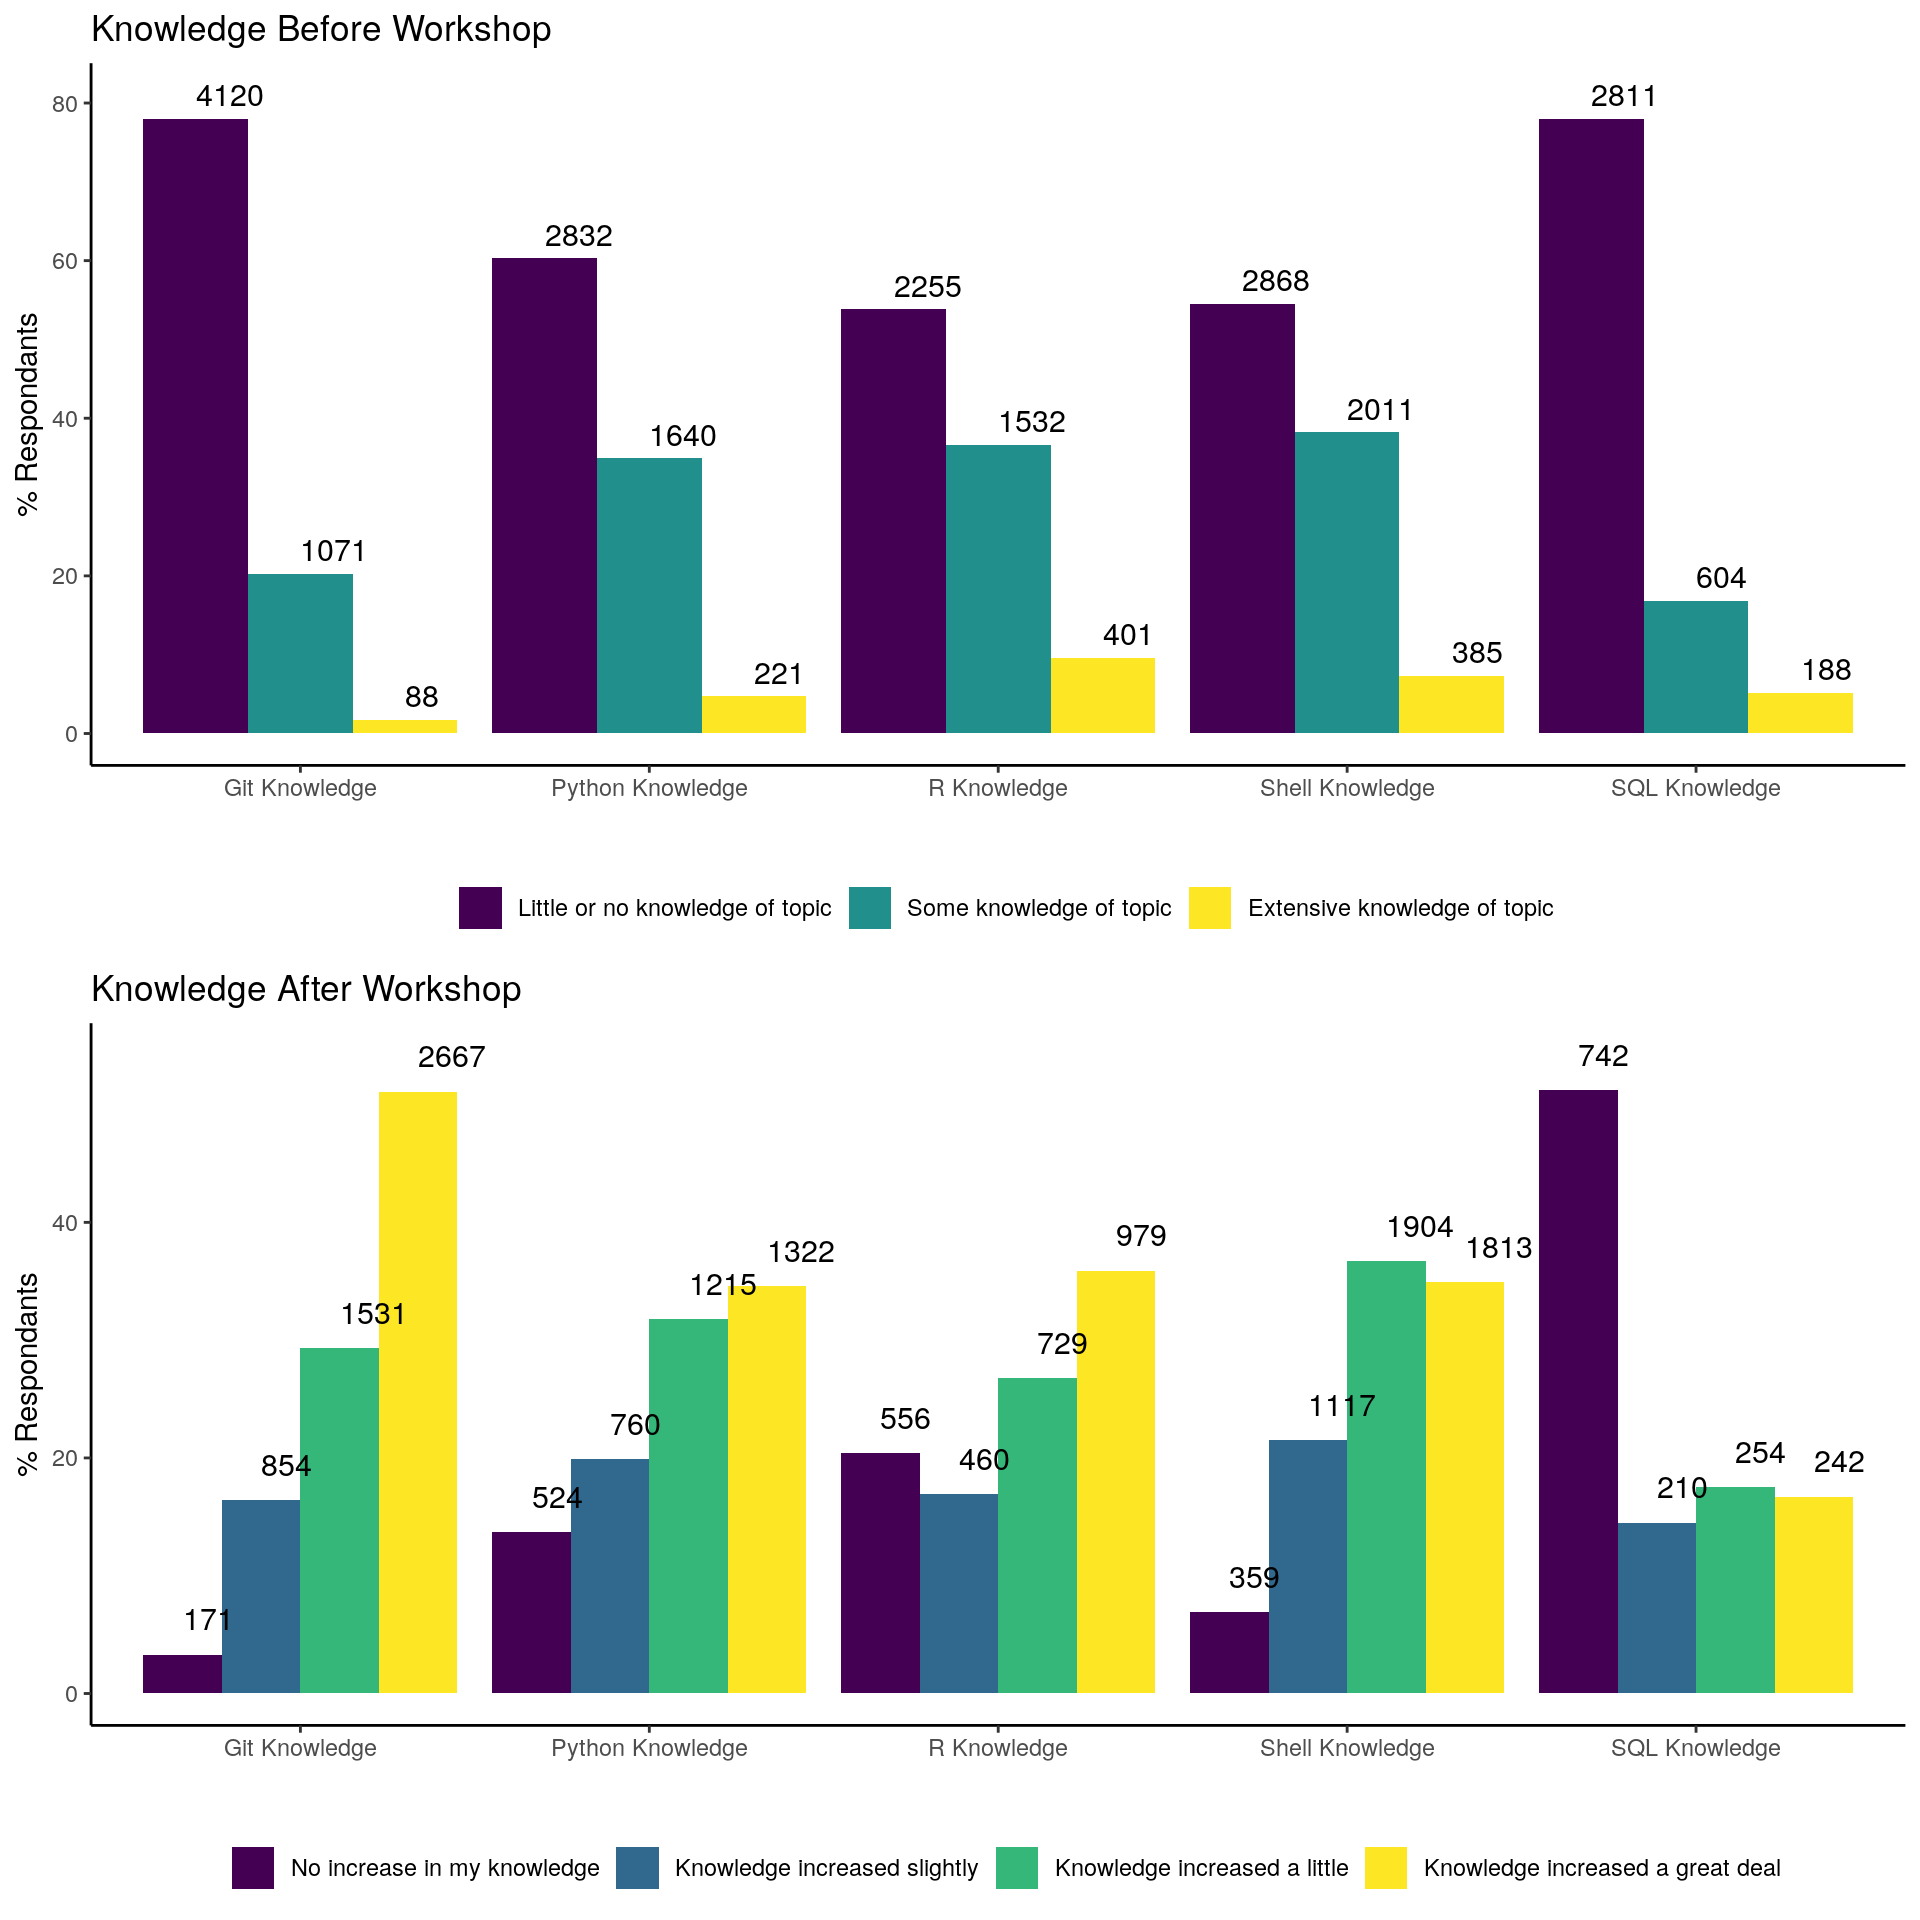
\includegraphics[width=\maxwidth]{../figures/swc-knowledge-change-1}

\subsubsection{Respondent Ability to Perform Computing
Tasks}\label{respondent-ability-to-perform-computing-tasks}

Motivation is important, but being confident in your ability to complete
specific computing tasks is an equally important goal of Software
Carpentry. The grid below shows respondents' self-reported ability to
complete tasks including:

\begin{itemize}
\tightlist
\item
  \textbf{Pipes}: Using pipes to connect shell commands
\item
  \textbf{Loops}: Writing a `for loop' to automate tasks\\
\item
  \textbf{Git}: Initializing a repository with git
\item
  \textbf{Function}: Writing a function
\item
  \textbf{Import Library}: Importing a library or package in R or Python
\item
  \textbf{Unit Test}: Writing a unit test in Python or R
\item
  \textbf{SQL Query}: Writing an SQL query
\end{itemize}

It also provides their self-reported level of confidence in being able
to complete the tasks above after completing the workshop.

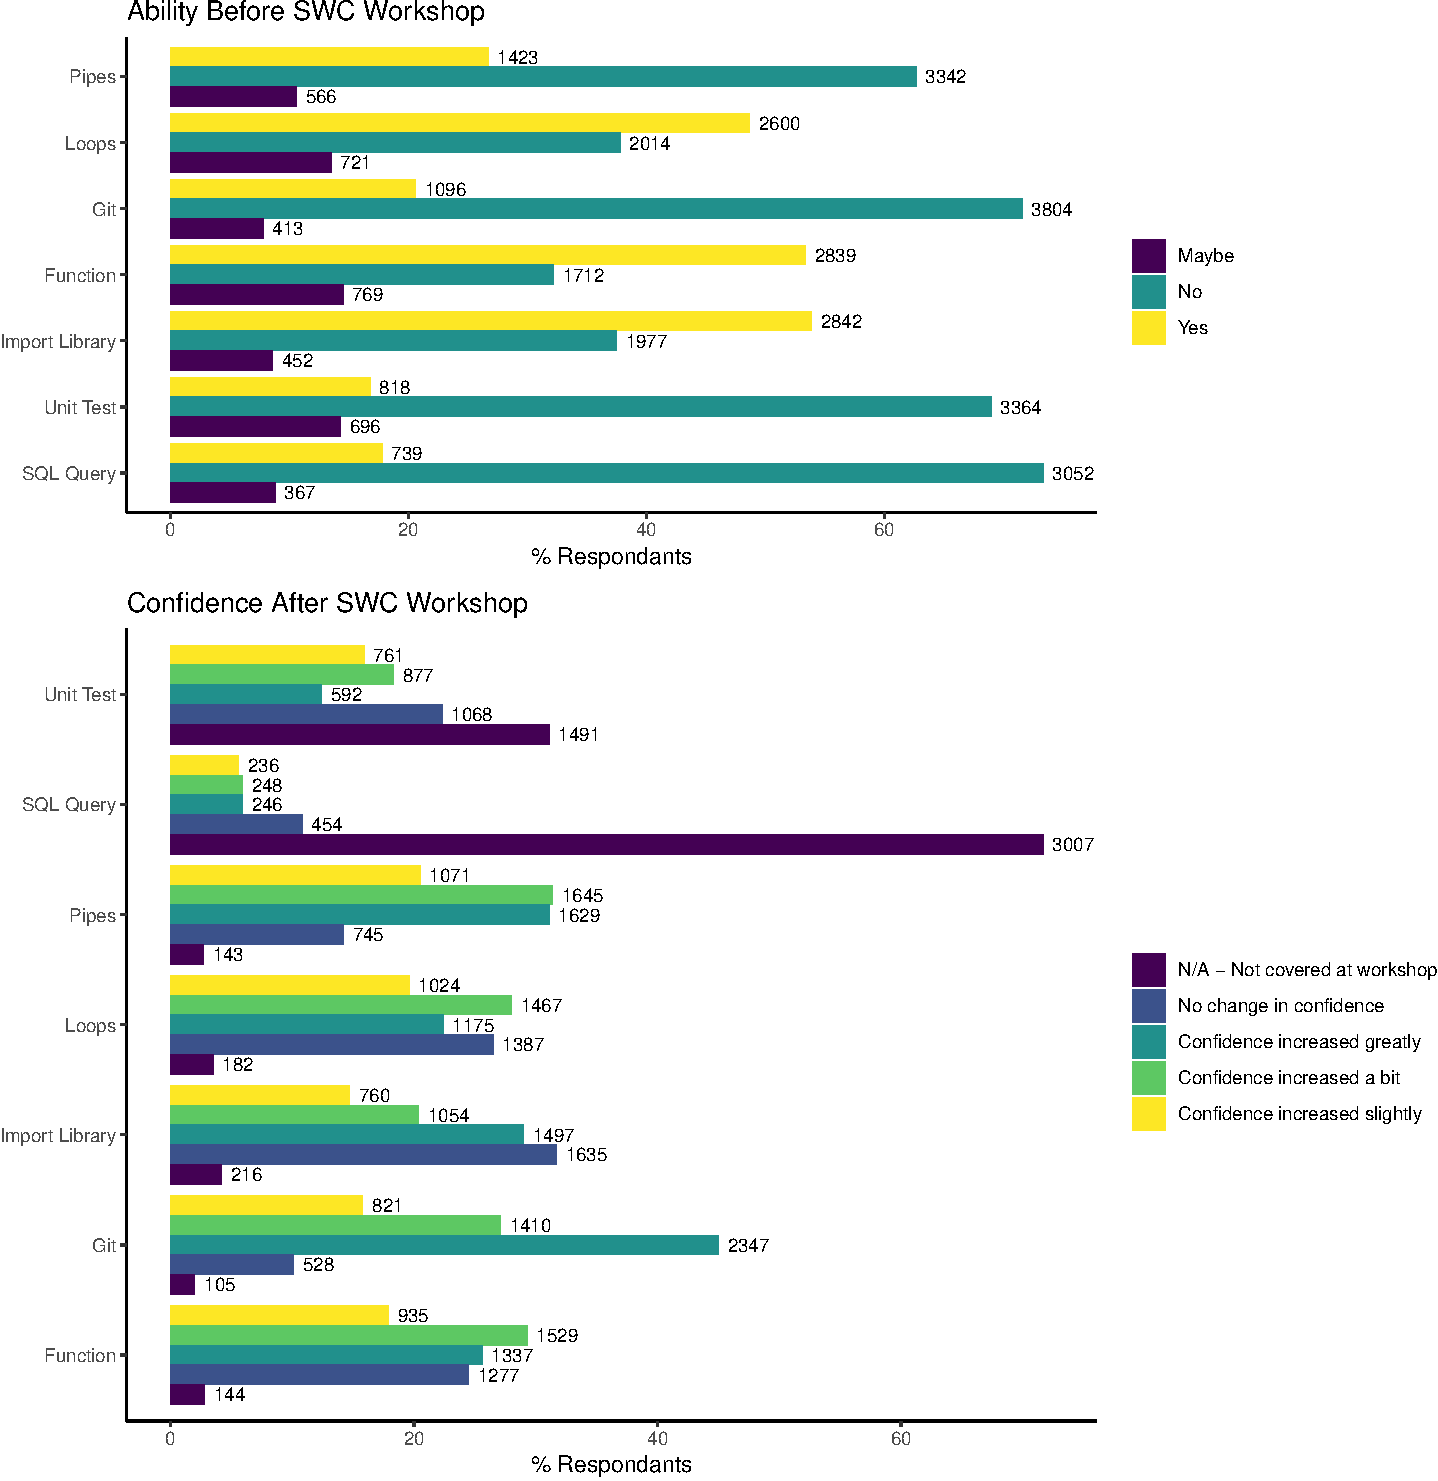
\includegraphics[width=\maxwidth]{../figures/swc-ability-confidence-1}

These figures tell us that, before the workshop, between 32.2\% and
73.4\% of the respondents did not feel they could initialize a
repository in Git, write a `for loop' to automate tasks, use pipes to
connect shell commands, write a SQL query, and/or write a unit test in R
or Python. 29\% of learners felt their confidence increased greatly with
respect to importing a library or package in R or Python. We consider
this significant as it is one of the fundamental skills that allows
learners to be successful in the other areas mentioned above.

In summary, respondents experienced increased confidence in their
ability to perform specific computing tasks and solve problems, or at
least search for answers to problems, as a result of participating in
Software Carpentry and Data Carpentry workshops.

\subsection{Demographics}\label{demographics}

\subsubsection{Countries}\label{countries}

The Carpentries is a global community that has recognized the importance
of bringing people to data through high-impact trainings. Though the
majority of Data Carpentry respondents report attendeding a workshop in
the United States of America (45.3\%), we also see that learners attend
workshops in African (e.g., Ethiopia 3.7\%) and European (e.g.,
Switzerland 0.6\%) countries. Note that we haven't held workshops in
Albania or Afghanistan, learners who selected these countries
interpreted this question to indicate their country of origin, or made a
mistake when selecting their answers.

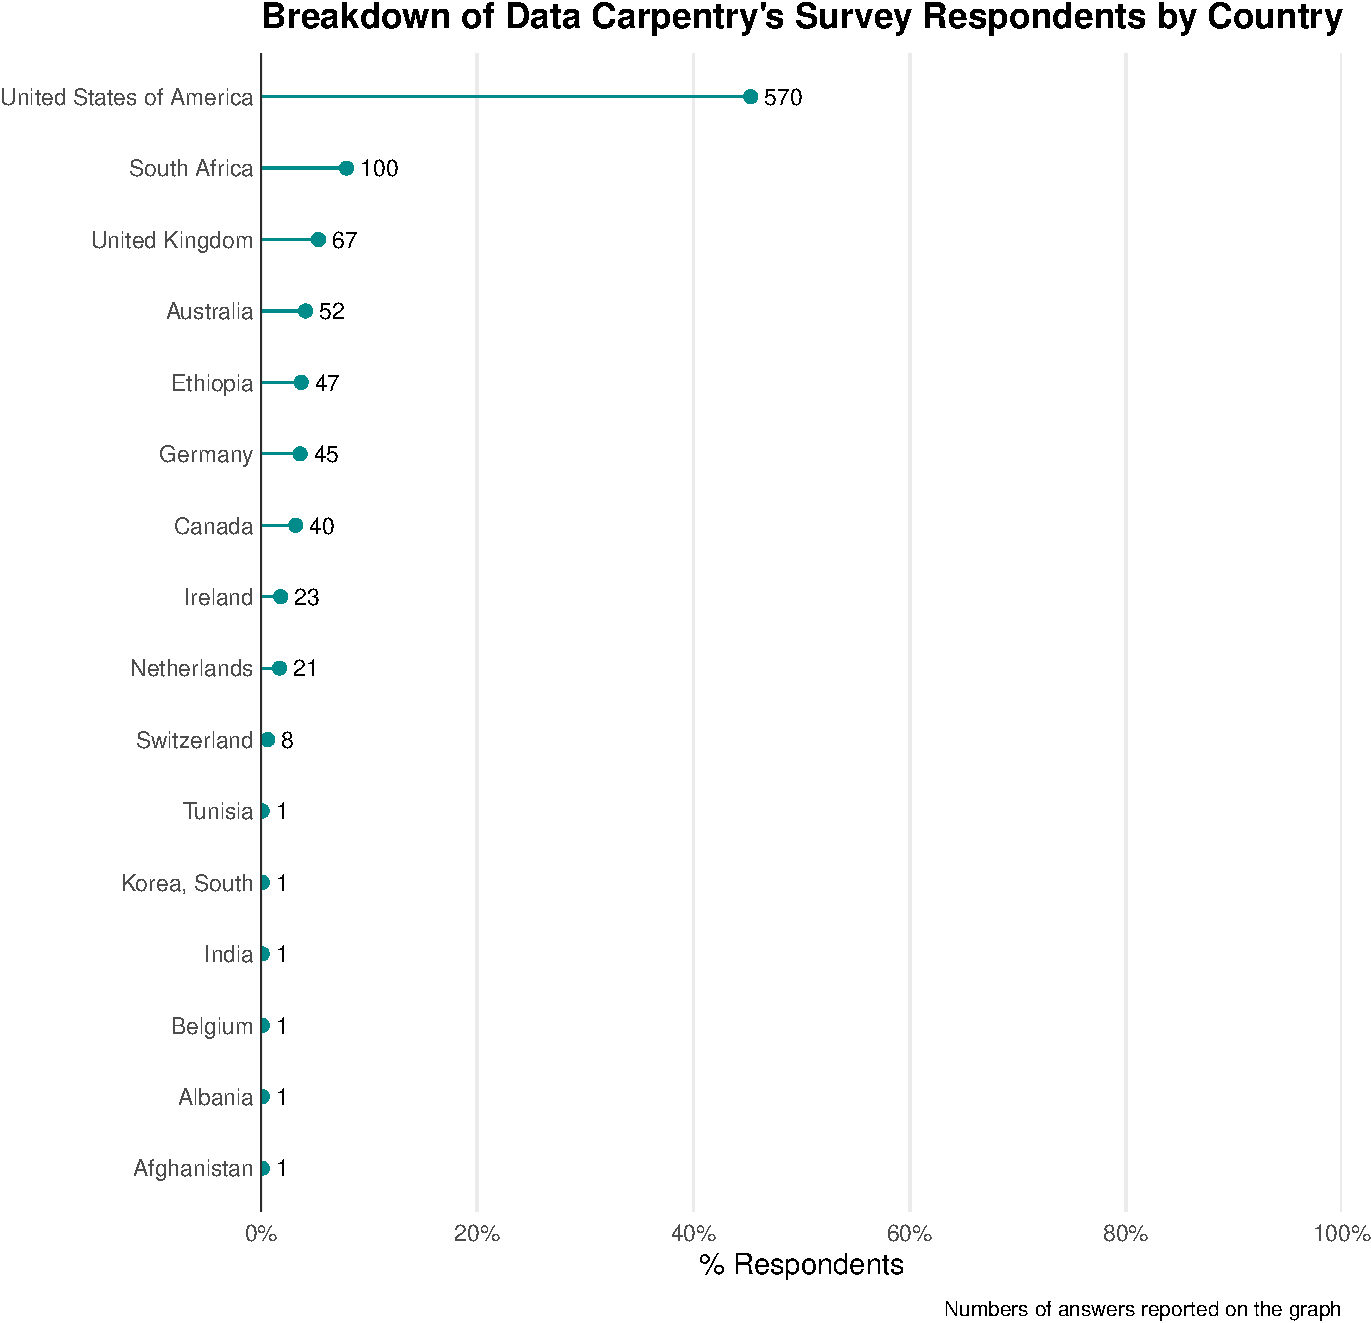
\includegraphics[width=\maxwidth]{../figures/dc-country-workshop-plot-1}

\begin{longtable}[]{@{}lrr@{}}
\toprule
Software Carpentry Workshops in US & n & \%\tabularnewline
\midrule
\endhead
Yes & 6468 & 45.7\tabularnewline
No & 4640 & 32.8\tabularnewline
Didn't answer & 3046 & 21.5\tabularnewline
\bottomrule
\end{longtable}

In Software Carpentry's pre-workshop survey, respondents are asked
whether or not their workshop will take place in the United States.
45.7\% of respondents attended a U.S. workshop.

\subsubsection{Learners' discipline}\label{learners-discipline}

\begin{longtable}[]{@{}lrr@{}}
\toprule
Data Carpentry's Respondents by Discipline & n & \%\tabularnewline
\midrule
\endhead
Life Sciences & 444 & 35.6\tabularnewline
Agricultural or Environmental Sciences & 307 & 24.6\tabularnewline
Bioinformatics/Genomics & 292 & 23.4\tabularnewline
Biomedical/Health Sciences & 288 & 23.1\tabularnewline
Other & 133 & 10.7\tabularnewline
Social Sciences & 122 & 9.8\tabularnewline
Mathematics or Statistics & 101 & 8.1\tabularnewline
Earth Sciences & 96 & 7.7\tabularnewline
Engineering & 91 & 7.3\tabularnewline
Computer Science & 88 & 7.1\tabularnewline
Business/Economics & 57 & 4.6\tabularnewline
Physical Sciences & 53 & 4.3\tabularnewline
Humanities & 53 & 4.3\tabularnewline
Library Sciences & 28 & 2.2\tabularnewline
\bottomrule
\end{longtable}

As previously mentioned, Data Carpentry's curricula is domain-specific
to Ecology, Genomics, Geospatial, and the Social Sciences. We see this
in the distribution of respondents by discipline. 35.6\% are in the Life
Science, while 24.6\%, 23.4\%, and 23.1\% are in Agricultural or
Environmental Sciences, Bioinformatics/Genomics, and Biomedical/Health
Sciences, respectively.

\begin{longtable}[]{@{}lrr@{}}
\toprule
\begin{minipage}[b]{0.81\columnwidth}\raggedright\strut
Software Carpentry's Respondents by Discipline\strut
\end{minipage} & \begin{minipage}[b]{0.05\columnwidth}\raggedleft\strut
n\strut
\end{minipage} & \begin{minipage}[b]{0.05\columnwidth}\raggedleft\strut
\%\strut
\end{minipage}\tabularnewline
\midrule
\endhead
\begin{minipage}[t]{0.81\columnwidth}\raggedright\strut
Life Science - Organismal/systems (ecology, botany, zoology,
microbiology, neuroscience)\strut
\end{minipage} & \begin{minipage}[t]{0.05\columnwidth}\raggedleft\strut
2694\strut
\end{minipage} & \begin{minipage}[t]{0.05\columnwidth}\raggedleft\strut
24.9\strut
\end{minipage}\tabularnewline
\begin{minipage}[t]{0.81\columnwidth}\raggedright\strut
Life Sciences (Genetics, genomics, bioinformatics )\strut
\end{minipage} & \begin{minipage}[t]{0.05\columnwidth}\raggedleft\strut
2680\strut
\end{minipage} & \begin{minipage}[t]{0.05\columnwidth}\raggedleft\strut
24.8\strut
\end{minipage}\tabularnewline
\begin{minipage}[t]{0.81\columnwidth}\raggedright\strut
Other\strut
\end{minipage} & \begin{minipage}[t]{0.05\columnwidth}\raggedleft\strut
1695\strut
\end{minipage} & \begin{minipage}[t]{0.05\columnwidth}\raggedleft\strut
15.7\strut
\end{minipage}\tabularnewline
\begin{minipage}[t]{0.81\columnwidth}\raggedright\strut
Mathematics/statistics\strut
\end{minipage} & \begin{minipage}[t]{0.05\columnwidth}\raggedleft\strut
940\strut
\end{minipage} & \begin{minipage}[t]{0.05\columnwidth}\raggedleft\strut
8.7\strut
\end{minipage}\tabularnewline
\begin{minipage}[t]{0.81\columnwidth}\raggedright\strut
Physics\strut
\end{minipage} & \begin{minipage}[t]{0.05\columnwidth}\raggedleft\strut
801\strut
\end{minipage} & \begin{minipage}[t]{0.05\columnwidth}\raggedleft\strut
7.4\strut
\end{minipage}\tabularnewline
\begin{minipage}[t]{0.81\columnwidth}\raggedright\strut
Planetary sciences (geology, climatology, oceanography, etc.)\strut
\end{minipage} & \begin{minipage}[t]{0.05\columnwidth}\raggedleft\strut
786\strut
\end{minipage} & \begin{minipage}[t]{0.05\columnwidth}\raggedleft\strut
7.3\strut
\end{minipage}\tabularnewline
\begin{minipage}[t]{0.81\columnwidth}\raggedright\strut
Civil, mechanical, chemical, or nuclear engineering\strut
\end{minipage} & \begin{minipage}[t]{0.05\columnwidth}\raggedleft\strut
692\strut
\end{minipage} & \begin{minipage}[t]{0.05\columnwidth}\raggedleft\strut
6.4\strut
\end{minipage}\tabularnewline
\begin{minipage}[t]{0.81\columnwidth}\raggedright\strut
Medicine and/or Pharmacy\strut
\end{minipage} & \begin{minipage}[t]{0.05\columnwidth}\raggedleft\strut
684\strut
\end{minipage} & \begin{minipage}[t]{0.05\columnwidth}\raggedleft\strut
6.3\strut
\end{minipage}\tabularnewline
\begin{minipage}[t]{0.81\columnwidth}\raggedright\strut
Social sciences\strut
\end{minipage} & \begin{minipage}[t]{0.05\columnwidth}\raggedleft\strut
591\strut
\end{minipage} & \begin{minipage}[t]{0.05\columnwidth}\raggedleft\strut
5.5\strut
\end{minipage}\tabularnewline
\begin{minipage}[t]{0.81\columnwidth}\raggedright\strut
Chemistry\strut
\end{minipage} & \begin{minipage}[t]{0.05\columnwidth}\raggedleft\strut
574\strut
\end{minipage} & \begin{minipage}[t]{0.05\columnwidth}\raggedleft\strut
5.3\strut
\end{minipage}\tabularnewline
\begin{minipage}[t]{0.81\columnwidth}\raggedright\strut
Economics/business\strut
\end{minipage} & \begin{minipage}[t]{0.05\columnwidth}\raggedleft\strut
481\strut
\end{minipage} & \begin{minipage}[t]{0.05\columnwidth}\raggedleft\strut
4.5\strut
\end{minipage}\tabularnewline
\begin{minipage}[t]{0.81\columnwidth}\raggedright\strut
Psychology\strut
\end{minipage} & \begin{minipage}[t]{0.05\columnwidth}\raggedleft\strut
417\strut
\end{minipage} & \begin{minipage}[t]{0.05\columnwidth}\raggedleft\strut
3.9\strut
\end{minipage}\tabularnewline
\begin{minipage}[t]{0.81\columnwidth}\raggedright\strut
Library and information science\strut
\end{minipage} & \begin{minipage}[t]{0.05\columnwidth}\raggedleft\strut
373\strut
\end{minipage} & \begin{minipage}[t]{0.05\columnwidth}\raggedleft\strut
3.5\strut
\end{minipage}\tabularnewline
\begin{minipage}[t]{0.81\columnwidth}\raggedright\strut
High performance computing\strut
\end{minipage} & \begin{minipage}[t]{0.05\columnwidth}\raggedleft\strut
360\strut
\end{minipage} & \begin{minipage}[t]{0.05\columnwidth}\raggedleft\strut
3.3\strut
\end{minipage}\tabularnewline
\begin{minipage}[t]{0.81\columnwidth}\raggedright\strut
Humanities\strut
\end{minipage} & \begin{minipage}[t]{0.05\columnwidth}\raggedleft\strut
318\strut
\end{minipage} & \begin{minipage}[t]{0.05\columnwidth}\raggedleft\strut
2.9\strut
\end{minipage}\tabularnewline
\begin{minipage}[t]{0.81\columnwidth}\raggedright\strut
Education\strut
\end{minipage} & \begin{minipage}[t]{0.05\columnwidth}\raggedleft\strut
264\strut
\end{minipage} & \begin{minipage}[t]{0.05\columnwidth}\raggedleft\strut
2.4\strut
\end{minipage}\tabularnewline
\begin{minipage}[t]{0.81\columnwidth}\raggedright\strut
Space sciences\strut
\end{minipage} & \begin{minipage}[t]{0.05\columnwidth}\raggedleft\strut
161\strut
\end{minipage} & \begin{minipage}[t]{0.05\columnwidth}\raggedleft\strut
1.5\strut
\end{minipage}\tabularnewline
\bottomrule
\end{longtable}

Software Carpentry's respondent base also has a majority Life Sciences
base; however we also see representation from those working in
Psychology, High Performance Computing, and Chemistry.

\subsubsection{Learners' career stage}\label{learners-career-stage}

\begin{longtable}[]{@{}lrr@{}}
\toprule
Data Carpentry's Respondents by Career Stage & n & \%\tabularnewline
\midrule
\endhead
Graduate Student & 592 & 47.6\tabularnewline
Research Staff & 200 & 16.1\tabularnewline
Postdoctoral Researcher & 183 & 14.7\tabularnewline
Faculty & 101 & 8.1\tabularnewline
Government Employee & 80 & 6.4\tabularnewline
Other & 79 & 6.4\tabularnewline
Industry Employee & 49 & 3.9\tabularnewline
Undergraduate Student & 48 & 3.9\tabularnewline
Management/Administrator & 20 & 1.6\tabularnewline
Retired/Not Employed & 18 & 1.4\tabularnewline
\bottomrule
\end{longtable}

As many of The Carpentries' workshops are hosted on university or
college campuses and other research-based communities, it is no surprise
that the majority of respondents are Graduate Students (47.6\% - DC,
35.4\% - SWC), Research Staff (16.1\% - DC,9.6\% - SWC), and
Postdoctoral Researchers (1.4\% - DC, 12.3\% - SWC).

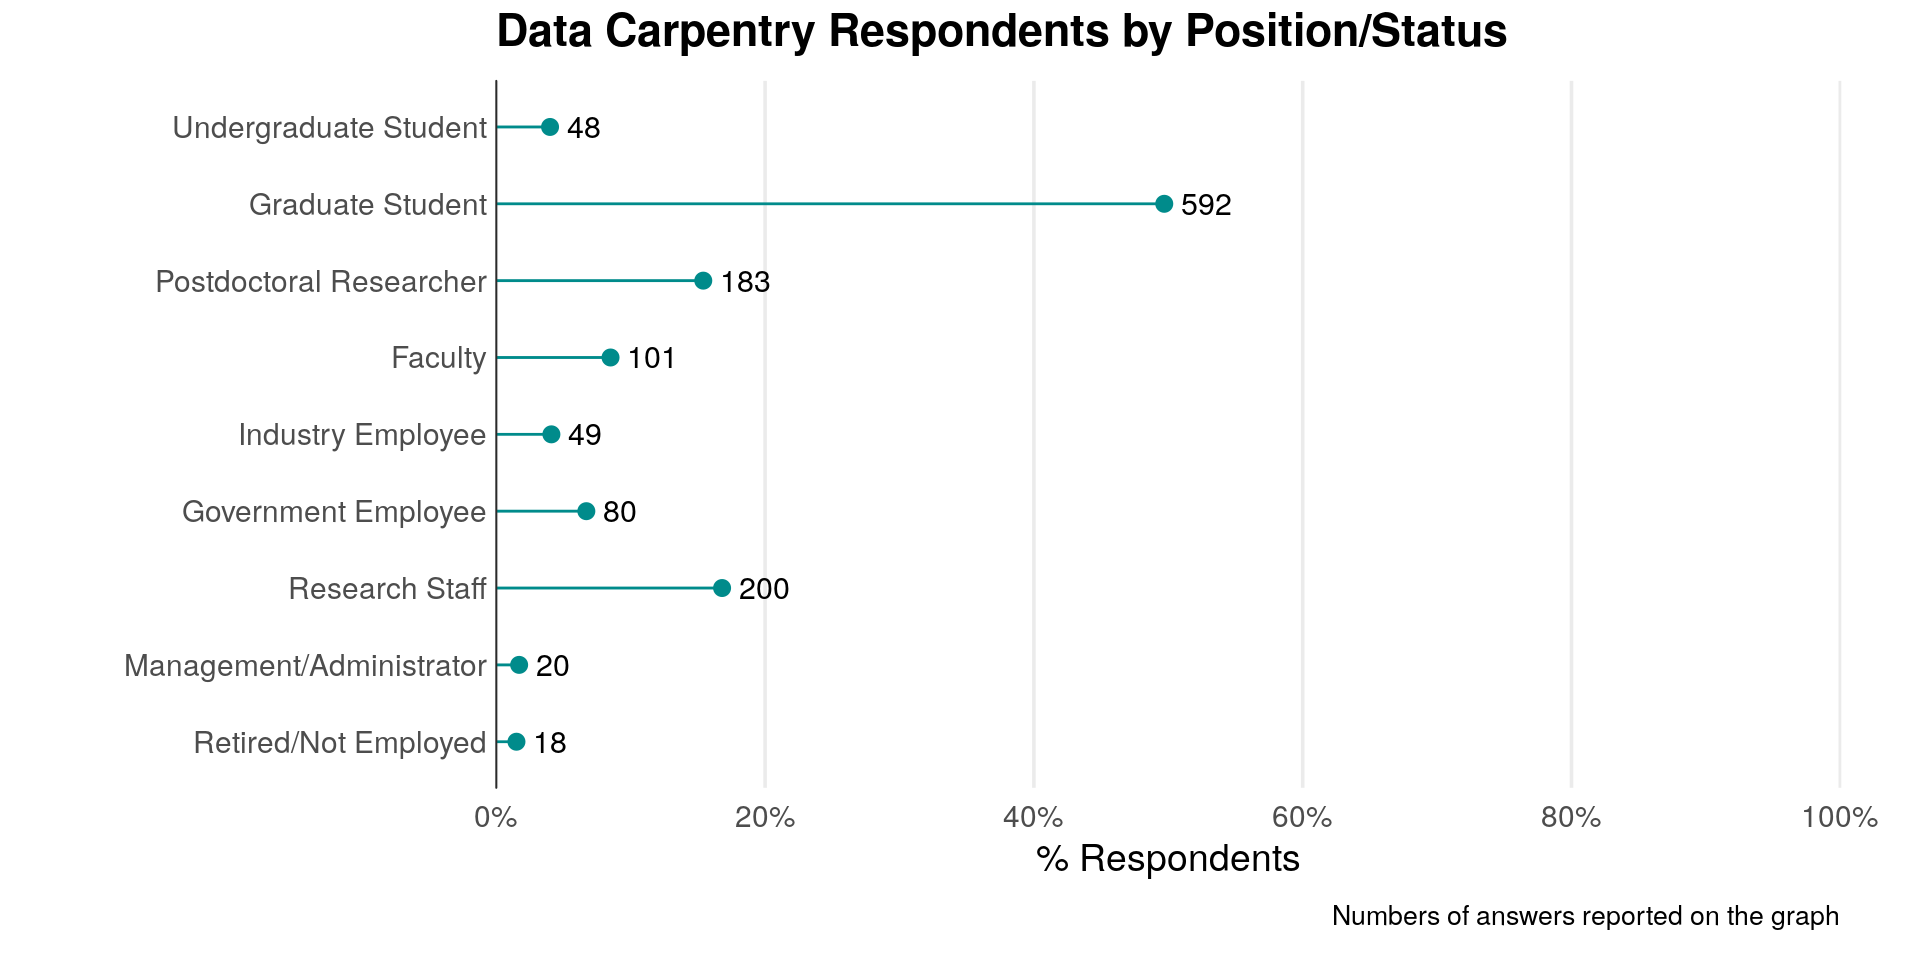
\includegraphics[width=\maxwidth]{../figures/dc-status-plot-1}

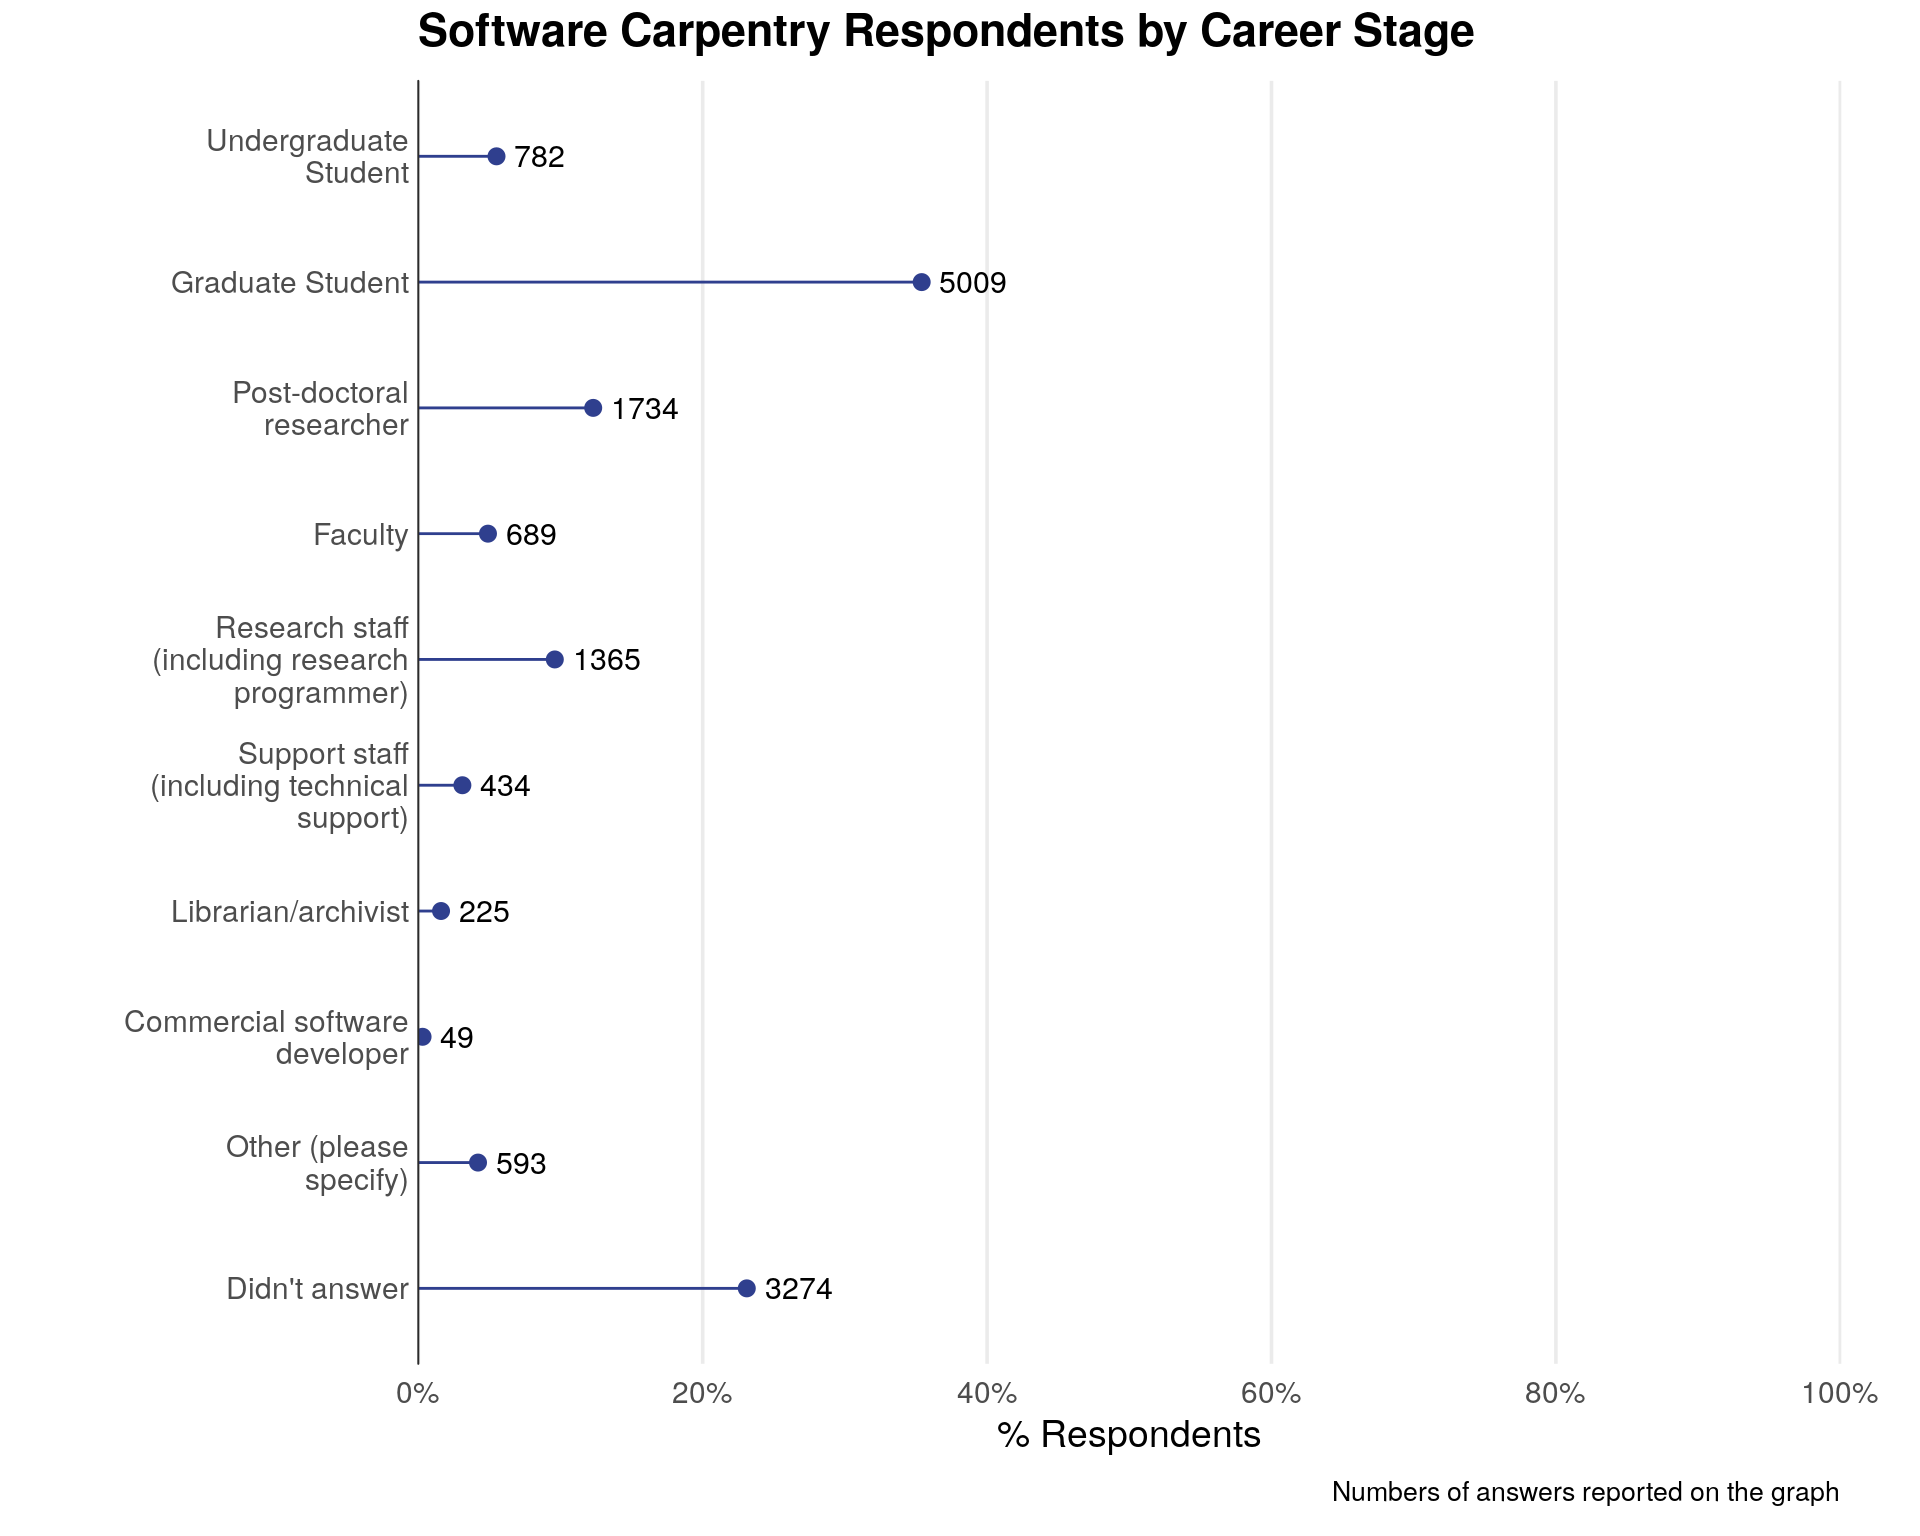
\includegraphics[width=\maxwidth]{../figures/swc-status-plot-1}

\subsubsection{Learners' operating
system}\label{learners-operating-system}

\begin{longtable}[]{@{}lrr@{}}
\toprule
Operating System Respondents Use in Data Carpentry Workshops & n &
\%\tabularnewline
\midrule
\endhead
Windows & 661 & 53.3\tabularnewline
Apple/Mac OS & 512 & 41.3\tabularnewline
UNIX/Linux & 50 & 4.0\tabularnewline
Not sure & 17 & 1.4\tabularnewline
\bottomrule
\end{longtable}

In our workshops, we recommend that learners use their own personal
laptop computers. It is important for learners to leave the workshop
with their own machine set up to do real work. Our instructors teach on
three major platforms: Windows, Mac OS X, and UNIX/Linux. We see a very
close representation of Windows (53.3\%) and Apple/Mac OS (41.3\%) users
in our Data Carpentry workshops, and even a few UNIX/Linux users (4\%).

\subsubsection{Gender and Racial/Ethnic
Identity}\label{gender-and-racialethnic-identity}

\begin{longtable}[]{@{}lrr@{}}
\toprule
Data Carpentry's U.S. Respondents' Gender Identity & n &
\%\tabularnewline
\midrule
\endhead
Female & 322 & 56.6\tabularnewline
Male & 223 & 39.2\tabularnewline
Transgender female & 2 & 0.4\tabularnewline
Transgender male & 0 & 0.0\tabularnewline
Gender variant/non-conforming & 0 & 0.0\tabularnewline
Prefer not to answer & 8 & 1.4\tabularnewline
Didn't answer & 14 & 2.5\tabularnewline
\bottomrule
\end{longtable}

\begin{longtable}[]{@{}lrr@{}}
\toprule
Data Carpentry's U.S. Respondents Racial/Ethnic Identity & n &
\%\tabularnewline
\midrule
\endhead
American Indian or Alaska Native & 4 & 0.7\tabularnewline
Asian & 152 & 27.7\tabularnewline
Black or African American & 25 & 4.6\tabularnewline
Hispanic or Latino(a) & 57 & 10.4\tabularnewline
Native Hawaiian or Other Pacific Islander & 3 & 0.5\tabularnewline
White & 316 & 57.6\tabularnewline
I prefer not to say. & 28 & 5.1\tabularnewline
Other & 8 & 1.5\tabularnewline
\bottomrule
\end{longtable}

\begin{longtable}[]{@{}lrr@{}}
\toprule
Software Carpentry's U.S. Respondents' Gender Identity & n &
\%\tabularnewline
\midrule
\endhead
Female & 3107 & 48.9\tabularnewline
Male & 3111 & 49.0\tabularnewline
Other & 18 & 0.3\tabularnewline
Prefer not to say & 115 & 1.8\tabularnewline
\bottomrule
\end{longtable}

\begin{longtable}[]{@{}lrr@{}}
\toprule
Software Carpentry's U.S. Respondents' Racial/Ethnic Identity & n &
\%\tabularnewline
\midrule
\endhead
American Indian or Alaskan Native & 29 & 0.5\tabularnewline
Asian / Pacific Islander & 1552 & 24.8\tabularnewline
Black or African American & 241 & 3.9\tabularnewline
Hispanic or Latino & 387 & 6.2\tabularnewline
Native Hawaiian or Other Pacific Islander & 5 & 0.1\tabularnewline
White / Caucasian & 3447 & 55.1\tabularnewline
Multiple ethnicity / Other (please specify) & 221 & 3.5\tabularnewline
Prefer not to say & 374 & 6.0\tabularnewline
\bottomrule
\end{longtable}

Gender and racial/ethnic identity information is collected for U.S.
participants, as we are keen to increase the number of diverse
instructors and learners we serve. Understanding our demographic makeup
helps us to understand what communities we reach and what programs we
should develop.

Currently, both Data (56.6\%) Carpentry and Software (48.9\%) Carpentry
see strong representation from women in the United States. Where we hope
to improve is in reaching the non-White audience, as fewer than 50.5\%
for Data Carpentry, and 45\% for SWC of our respondents are from
communities historically underrepresented in the science, technology,
engineering, and mathematics (STEM) fields.

\subsection{Summary}\label{summary}

This report focused on Data and Software Carpentry learners' skills,
perspectives, and experiences in workshops. Our two-day coding workshops
increase researchers' daily programming usage, and confidence in working
with open source tools. Currently, Data Carpentry and Software Carpentry
use different surveys to collect pre and post workshop data. In the
coming months, we plan to develop one common survey to be used for both
Data Carpentry and Software Carpentry.

For a comprehensive look at our workshops and instructor training, have
a look at our
\href{https://carpentries.github.io/assessment/programmatic-assessment/workshops/outputs/final_report.html}{programmatic
assessment report}.


\end{document}
